\chapter[Intégration complexe]{Intégration des fonctions d'une variable complexe}
Le sujet de l'intégration d'une fonction dans le plan complexe peut être abordé de plusieurs manières, notamment à l'aide des sommes de Riemann. Par contre, une question se pose : si nous intégrons une fonction le long d'un chemin $\gamma$ à partir d'un point $\gamma(a)$ vers un point $\gamma(b)$, la valeur de l'intégrale dépend-elle uniquement des points de départ et d'arrivée de $\gamma$ (auquel cas on peut faire le parallèle avec le cas réel $\int_a^b f(x) dx = F(b) - F(a)$, $F$ étant une primitive de $f$), ou dépend-elle de $\gamma(a)$, $\gamma(b)$ \textbf{et} de $\gamma$ ? Nous aurons la réponse dans ce chapitre avec notamment les formules de Cauchy.

\section{Intégration le long d'un chemin}



% \begin{defn}
% Si $E$ est un espace vectoriel, une forme linéaire (ou covecteur) est une application linéaire de $E$ dans $\R$ ou $\C$
% \end{defn}

% \begin{defn}
% Si $E$ est un espace vectoriel, l'ensemble des formes linéaires sur $E$ est un espace vectoriel appelé dual de $E$, noté $E^*$ 
% \end{defn}

% \begin{defn}
% Si $E$ est un espace vectoriel de dimension finie et $U$ un ouvert de $E$, une forme différentielle de degré 1 (appelée aussi 1-forme) et de classe $C^\infty$ est une application $\omega \colon U \to E^*$ de classe $C^\infty$
% \end{defn}

% Une forme différentielle de degré 1 peut être vue comme un champ de formes linéaires : à chaque point d'un ouvert $U$, on fait correspondre une forme linéaire.


% Toute application continue $f \colon U \to \C$, définit deux formes différentielles de degré $1$ : $f \diff z$ et $f \diff \bar{z}$. Néanmoins, selon la définition d'une $1$-forme, il faut supposer $f$ de classe $C^\infty$. En fait, il est toujours possible de définir des formes différentielles de classe $C^k$, pour un $k$ suffisamment grand sans changer les résultats précédents. %(il faudra par exemple $k \geq 1$, si l'on veut calculer la différentielle extérieure d'une $0$ ou d'une $1$-forme).

\begin{fdefn}
\label{def:integration_chemin}
Soit $U$ un ouvert de $\C$ et $f \colon U \to \C$ une application continue. Soit $\gamma \colon [a,b] \to U$ un chemin de classe $C^1$. 
L'intégrale de $f$ le long de $\gamma$ sera définie comme:
\[
\int_{\gamma}f \diff z = \int_{[a,b]}f\left(\gamma(t)\right)\gamma^\prime(t)\diff t
\]
\end{fdefn}
\begin{rem}
On peut également définir l'intégrale par rapport à $\diff \bar{z}$ comme:
\[
\int_{\gamma}f \diff \bar{z} = \int_{[a,b]}f\left(\gamma(t)\right)\overline{\gamma^\prime(t)} \diff t
\]
\end{rem}

Nous allons appliquer cette définition pour calculer une intégrale très simple : celle de la fonction inverse sur le cercle unité.
\begin{exercice} \label{ex:int_1surz}
Soit la fonction :
\[f(z)= \frac{1}{z}
\]
Calculer son intégrale sur le cercle unité $C(0,1) = \{ z \in \C \, | \, \| z \| = 1 \}$ que l'on pourra par exemple paramétrer par
\begin{align*}
    \gamma \colon [0;1] & \to \C \\
                     t  & \mapsto e^{2 \pi i t}
\end{align*}
Plus généralement, calculer l'intégrale de $f$ sur $\gamma_R = \{ z \in \C \, | \, \| z \| = R \}$ avec $R > 0$. Que remarque-t-on ?

Enfin, calculer l'intégrale de $f$ sur le contour $- \gamma : t \in [0;1] \mapsto e^{-2 \pi i t}$
\end{exercice}

Un autre point de vue consiste à traduire l'intégrale $\int_{\gamma}f \diff z$ en se ramenant aux notions physiques de \textbf{flux} et de \textbf{travail}.
Si $f=u + i v$ et $\gamma(t)=x(t) + i y(t)$, alors
\[\int_{\gamma}f \diff z =\int_{[0,1]} \left(\, u(\gamma(t))\, x^\prime(t) - v(\gamma(t))\, y^\prime(t)\, \right) \diff t + i \int_{[0,1]} \left(\, u(\gamma(t))\, y^\prime(t) + v(\gamma(t))\, x^\prime(t)\, \right) \diff t.\]

Introduisons le repère mobile, sur le chemin $\gamma$, constitué du vecteur tangent unitaire $T$ et du vecteur normal unitaire $N$, orienté vers la droite lorsque l'on parcourt le chemin (cf. figure~\ref{fig:repere}) ; plus précisément
\[T(t)=\frac{\gamma^\prime(t)}{\lvert\gamma^\prime(t)\rvert} = \frac{1}{\lvert\gamma^\prime(t)\rvert}\begin{pmatrix} x'(t) \\ y'(t) \end{pmatrix}, \quad T(t)=i \, N(t), \text{ donc } N(t) = \frac{1}{\lvert\gamma^\prime(t)\rvert}\begin{pmatrix}y'(t) \\ -x'(t)\end{pmatrix}\]


\begin{figure}[ht]
\begin{center}
\begin{tikzpicture}[line cap=round,line join=round,>=triangle 45,x=1.0cm,y=1.0cm, scale=0.8]
  \tikzset{
  % style to apply some styles to each segment of a path
  on each segment/.style={
    decorate,
    decoration={
      show path construction,
      moveto code={},
      lineto code={
        \path [#1]
        (\tikzinputsegmentfirst) -- (\tikzinputsegmentlast);
      },
      curveto code={
        \path [#1] (\tikzinputsegmentfirst)
        .. controls
        (\tikzinputsegmentsupporta) and (\tikzinputsegmentsupportb)
        ..
        (\tikzinputsegmentlast);
      },
      closepath code={
        \path [#1]
        (\tikzinputsegmentfirst) -- (\tikzinputsegmentlast);
      },
    },
  },
  % style to add an arrow in the middle of a path
  mid arrow/.style={postaction={decorate,decoration={
        markings,
        mark=at position .5 with {\arrow[#1]{stealth}}
      }}},
}   
 
\node (A) at (1.86,-3.1) {};
\node (B) at (3.9,0.52){};
\node (C) at (4.36, 3.4){}; 
\draw[blue] plot [smooth,tension=1]  
    coordinates {(A)  (B) (C)}[postaction={on each segment={draw,-{latex[red]}}}];
\draw [->,line width=1.2pt] (B) -- (4.8096345814716885,2.9879293140889756) node[near end, right=0.1] {{\large $T$}};
\draw [->,line width=1.2pt] (B) -- (6.343272843835928,-0.3805466477650137)node[near end, above ] {{\large $N$}};
%\draw [->,line width=1.2pt] (B) -- (2.230,1.4)node[near end, above ] {{\large $n$}};
\draw [fill=blue] (B) circle (2.5pt);
\end{tikzpicture}
\caption{Repère mobile sur un chemin.} \label{fig:repere}
\end{center}
\end{figure}

Associons à la fonction $f = u + i v$, le champ de vecteurs $H=(u,-v)$ ($H$ est appelé champ de vecteurs de \textit{Pólya}), alors 
\begin{align*}
\int_{\gamma}f \diff z &= \int_0^1 \langle \, H(\gamma(t)), T(t) \, \rangle \, \lvert\gamma^\prime(t)\rvert\diff t +  i \int_0^1 \langle \, H(\gamma(t)), N(t) \, \rangle \, \lvert\gamma^\prime(t)\rvert\diff t \\
%&= \int_0^1 \langle \, H(\gamma(t)), T(t) \, \rangle \, \lvert\gamma^\prime(t)\rvert\diff t +  i \int_0^1 \langle \, H(\gamma(t)), N(t) \, \rangle \, \lvert\gamma^\prime(t)\rvert\diff t
\end{align*}

Nous reconnaissons :
\begin{itemize}
    \item[$\bullet$] dans le premier terme de droite, le travail du champ $H$ le long du chemin $\gamma$ (assimilable au travail d'une force, par exemple)
    \item[$\bullet$] dans le second terme de droite, le flux du champ $H$ à travers $\gamma$ (assimilable au flux d'un fluide ou d'un champ électrique)
\end{itemize} 

Ainsi, l'intégrale complexe regroupe ces deux termes très utilisés en physique. Notons aussi l'interprétation possible d'une fonction complexe en termes de champ de vecteurs dans $\R^2.$
\begin{fprop}[Changement de variable]
\label{prop:changement_variable}
Soit $U$ un ouvert de $\C$, $\gamma \colon [a,b] \to U$ un chemin de classe $C^1$ et $\phi$ un $C^1$-difféomorphisme de $U$ sur $\phi(U)$. Pour $f$ application continue définie sur $\phi(U)$ on a:
\[
\int_{\phi(\gamma)} f(z) dz = \int_{\gamma} f \circ \phi (z) \phi^\prime(z) dz
\]
\end{fprop}
\begin{proof}
    Par définition:
    \[
\int_{\gamma} f \circ \phi (z) \phi^\prime(z) dz = \int_a^b f \circ \phi \left( \gamma(t) \right) \phi^\prime\left(
\gamma(t) \right) \gamma^\prime(t) dt
    \]
    Or $ \phi^\prime\left(
\gamma(t) \right) \gamma^\prime(t) = \left( \phi \circ \gamma \right)^\prime(t)$, d'où:
\[
\int_{\gamma} f \circ \phi (z) \phi^\prime(z) dz = \int_a^b f \circ \phi \left( \gamma(t) \right)\left( \phi \circ \gamma \right)^\prime(t) dt = \int_{\phi \circ \gamma} f(z) dz
    \]
\end{proof}

\begin{fprop}
Soit $U$ un ouvert de $\C$ et soit $F \colon U \to \C$ une application holomorphe de dérivée continue $f$. Soit $\gamma \colon [a,b] \to U$ un chemin de classe $C^1$. On a:
\[
\int_\gamma f(z) dz = F(\gamma(b)) - F(\gamma(a))
\]
\end{fprop}
\begin{proof}
Il suffit de remarquer que:
\[
\frac{d}{dt}F\circ \gamma(t) = f(\gamma(t)) \gamma^\prime(t)
\]
et d'appliquer la formule de la définition \ref{def:integration_chemin}.
\end{proof}
\begin{rem}
L'application $F$ est appelée une primitive de $f$. Elle est définie à une constante additive près. On remarque que lorsqu'une application continue admet une primitive, son intégrale sur tout lacet contenu dans $U$ est nulle. 
\end{rem}
En analyse complexe, il est commode d'introduire la longueur d'arc infinitésimale $ds = \lvert \diff z \rvert =\lvert\gamma^\prime(t)\rvert\diff t$ de sorte que
\[\int_ \gamma f(z) \lvert \diff z \rvert = \int_{[0,1]} f(\gamma(t)) \lvert\gamma^\prime(t)\rvert \diff t .\]
\begin{fprop}[Inégalité triangulaire et inégalité ML]
Soit $\gamma$ un chemin de classe $C^1$ par morceaux et soit $f$ une application  intégrable le long de $\gamma$. Alors~:
\[
\Bigl \lvert\int_{\gamma} f(z) dz\Bigr \rvert \leq \int_{\gamma} \lvert f(z) \rvert \lvert dz \rvert.
\]
De plus si $\gamma$ a pour longueur $L$ et $\lvert f(z) \rvert \leq M$ sur $\gamma$ (qui est compact), alors
\[
\Bigl \lvert\int_{\gamma} f(z) dz\Bigr \rvert \leq M L.
\]
\end{fprop}
On peut obtenir facilement ce résultat en utilisant les sommes de Riemann-Stieltjes.
Cette majoration est utilisée pour obtenir un résultat très utile en
pratique~: le lemme de Jordan.

%\begin{fprop}(Lemme de Jordan)\label{prop:jordan}
%Soit $\gamma_r$ le chemin formé d'un arc de cercle de rayon $r$, de centre $z_0$ parcouru
% dans le sens trigonométrique, d'angle initial $\alpha_0$ et d'angle final
% $\alpha_1$. Soit $f$ une application continue sur $\gamma_r$, pour
% tout $r>0$. Si la borne supérieure de l'application $\lvert (z-z_0)f(z)\rvert$ ($z \in \gamma_r$) tend vers $0$ lorsque $r \to 0$ 
% (resp. $r \to +\infty$), alors~:
%\[
%\lim_{\substack{r \to 0^+ \\(\text{resp.} r \to  +\infty)}} \int_{\gamma_r} f(z) dz = 0.
%\]
%\end{fprop}
%
%
%\begin{proof}
%\ 
%
%\begin{minipage}{0.3\linewidth}
%\begin{center}
%\begin{tikzpicture}[line cap=round,line join=round,>=triangle 45,x=1.0cm,y=1.0cm, scale=0.5]
%\clip(-0.5,-0.7) rectangle (7,7.);
%\draw [shift={(0.,0.)},line width=1.2pt,color=gray,fill=gray,fill opacity=0.10000000149011612] (0,0) -- (0.:0.66) arc (0.:18.43494882292201:0.66) -- cycle;
%\draw [shift={(0.,0.)},line width=1.2pt,color=gray,fill=gray,fill opacity=0.10000000149011612] (0,0) -- (0.:0.66) arc (0.:71.56505117707799:0.66) -- cycle;
%\draw [color=pblue, shift={(0.,0.)},line width=1.2pt]  plot[domain=0.32175055439664224:1.2490457723982544,variable=\t]({1.*6.324555320336759*cos(\t r)+0.*6.324555320336759*sin(\t r)},{0.*6.324555320336759*cos(\t r)+1.*6.324555320336759*sin(\t r)});
%\begin{scriptsize}
%\draw[color=black] (4.665636363636368,4.813) node {{\normalsize $\gamma_r$}};
%\draw[color=blue] (1.5,0.204) node {{\normalsize$\alpha_0$}};
%\draw[color=blue] (1.2,1) node {{\normalsize $\alpha_1$}};
%\draw [fill=pblue] (0,0) circle (2.5pt);
%\draw (0,-0.5) node {{\normalsize $z_0$}};
%\draw (0,0) -- (6,2);
%\draw (0,0) -- (2,6);
%\draw (0,0) -- (6,0);
%\end{scriptsize}
%\end{tikzpicture}
%\end{center}
%\end{minipage}
%\begin{minipage}{0.70\linewidth}
%Pour $r$ fixé, le chemin $\gamma_r$ s'exprime par:
%\[
%\gamma_r \colon t \in [0,1] \mapsto z_0 + r e^{i \left(\alpha_0 +
%t (\alpha_1 - \alpha_0)\right)}
%\]
%On a donc $\lvert \diff z \rvert= (\alpha_1-\alpha_0) r \diff t$, d'où :
%\[
%\left|\int_{\gamma_r} f(z) dz\right| \leq (\alpha_1-\alpha_0) r  \int_0^1
%\lvert f(\gamma_r(t))
%\rvert \diff t 
%\]
%On remarque par ailleurs que $|(z-z_0)f(z)|=r|f(z)|$ pour $z$ appartenant à
%l'image de $\gamma_r$. La conclusion du théorème s'obtient alors directement.
%\end{minipage}
%\end{proof}
%
%Une formulation du lemme de Jordan, très utile dans le calcul des intégrales complexes est la suivante~:
\begin{fprop}(Lemme de Jordan)\label{prop:jordan}
Soit $\gamma_r =\{r e^{i \theta} : \theta \in [0,\pi]\}$ le demi-cercle de rayon $r$, centré en zéro, situé dans le demi-plan supérieur. Soit $f$ une application continue sur $\gamma_r$ de la forme 
\[f(z)=g(z) e^{i a z}, \quad z \in \gamma_r,\]
avec $a$ un réel strictement positif. Soit $M_r=\max_{\theta \in [0, \pi]} \lvert g\left(re^{i\theta}\right)\rvert$, alors
\[\Bigl \lvert\int_{\gamma_r} f(z) \diff z \Bigr \rvert \leq \frac{\pi}{a}M_r.\] 
\end{fprop}
\begin{rem}
En particulier, si $f$ est continue sur $\gamma_r$ pour tout $r>0$ et si $\lim_{r \to \infty} M_r=0$ (resp. $\lim_{r \to 0} M_r=0$), alors
\[\lim_{\substack{r \to \infty \\(\text{resp.} r \to  0)}} \int_{\gamma_r} f(z)\diff z =0.\]
\end{rem}
\begin{proof}
D'après les hypothèses, nous avons 
\[\Bigl \lvert\int_{\gamma_r} f(z) \diff z \Bigr \rvert \leq r M_r \int_0^\pi e^{- a r \sin \theta} \diff \theta = 2 r M_r \int_0^{\pi/2} e^{- a r \sin \theta} \diff \theta.\]
La fonction $\sin$ étant concave sur $[0,\pi/2]$, son graphe est au-dessus du segment rejoignant les extrémités, d'où $\sin \theta \geq 2 \theta/\pi$. Nous en déduisons que 
\[ \Bigl \lvert\int_{\gamma_r} f(z) \diff z \Bigr \rvert \leq 2 r M_r \int_0^{\pi/2} e^{-2 a r \theta/\pi} \diff \theta
=\frac{\pi}{a} (1-e^{-a r}) M_r \leq \frac{\pi}{a}M_r.\]
\end{proof}

\section{Primitives locales}

Les résultats de cette section sont fondamentaux pour la suite. Ils vont
permettre en particulier d'établir que toute application holomorphe dans un
domaine y est en fait analytique.

\subsection{Quelques considérations sur les domaines du plan}
Rappelons qu'un domaine $\Omega \subset \C$ est un ouvert connexe non vide de $\C$ (donc connexe par arcs en vertu de la proposition \ref{prop:ouvert_connexe}).  Le disque unité $B(0 ;1)$ privé de l'origine est un domaine du plan qui se distingue du disque unité par la présence d'un \og trou \fg{}. La différence jouera un rôle très important dans le calcul des intégrales complexes. La notion d'homotopie donne un cadre formel permettant de caractériser la topologie des domaines du plan.

\begin{fdefn}(Homotopie)
Soit $\Omega \subset \mathbb{C}$, $\gamma_1, \gamma_2$ deux chemins de $\Omega$ et $I$ une partie de $[0,1]$ telle que $\forall t \in I, \, \gamma_1(t) = \gamma_2(t)$. On dira que $\gamma_1$ et $\gamma_2$ sont homotopes relativement à $I$ s'il existe une application continue:
\[
H \colon [0,1] \times [0,1] \to \Omega
\] 
telle que:
\begin{itemize}
\item $\forall t \in [0,1], \, H(0,t) = \gamma_1(t), \, H(1,t) = \gamma_2(t)$
\item $\forall s \in [0,1], \, \forall t \in I, H(s,t) = \gamma_1(t)$
\end{itemize}
\end{fdefn}
\begin{rem}
Le cas le plus fréquemment rencontré est $I=\{0,1\}$. On parle alors d'homotopie à extrémités fixées.
\end{rem}
On définira également la notion d'homotopie entre lacets.
\begin{fdefn}(Homotopie de lacets)
Soit $\Omega \subset \mathbb{C}$ et  $\gamma_1, \gamma_2$ deux
lacets de $\Omega$. Soit $I$ une partie de $[0,1]$ telle que $\forall t \in I, \, \gamma_1(t)=\gamma_2(t)$.
On dira que $\gamma_1$ et $\gamma_2$ sont homotopes relativement à $I$ s'il existe une application continue:
\[
H \colon [0,1] \times [0,1] \to \Omega
\] 
telle que:
\begin{itemize}
\item $\forall t \in [0,1], \, H(0,t) = \gamma_1(t), \, H(1,t) = \gamma_2(t)$
\item $\forall s \in [0,1], \, H(s,0) = H(s,1)$
\item $\forall t \in I, \forall s \in [0,1], \, H(s,t)=\gamma_1(t)$
\end{itemize}
\end{fdefn}
Pour chaque $s\in [0,1]$, l'application $\gamma_s(t)=H(s,t)$ est un chemin d'extrémités $\gamma_1(0)$ et $\gamma_1(1)$ d'image incluse dans $\Omega$. Pour $t$ fixé, on passe continûment de $\gamma_1(t)$ à $\gamma_2(t)$ par l'application $H(\cdot, t) \colon s \mapsto H(s,t)$, tel que représenté en figure \ref{fig:exemple_homotopie}.
\begin{figure}[h]

\begin{center}
\shorthandoff{!}\shorthandoff{:}
\begin{tikzpicture}
\clip(5,0) rectangle (15,5);
 \tikzset{
  % style to apply some styles to each segment of a path
  on each segment/.style={
    decorate,
    decoration={
      show path construction,
      moveto code={},
      lineto code={
        \path [#1]
        (\tikzinputsegmentfirst) -- (\tikzinputsegmentlast);
      },
      curveto code={
        \path [#1] (\tikzinputsegmentfirst)
        .. controls
        (\tikzinputsegmentsupporta) and (\tikzinputsegmentsupportb)
        ..
        (\tikzinputsegmentlast);
      },
      closepath code={
        \path [#1]
        (\tikzinputsegmentfirst) -- (\tikzinputsegmentlast);
      },
    },
  },
  % style to add an arrow in the middle of a path
  mid arrow/.style={postaction={decorate,decoration={
        markings,
        mark=at position .5 with {\arrow[#1]{stealth}}
      }}},
}   
 
  %\node at (0,0) {$F : I \times I \rightarrow X$};
  \node  (x1) at (6,0)  {$\bullet$};
  \node  (x0) at (9,4)  {$\bullet$}; 
  \draw[line width=1.2pt,color=blue,postaction={on each segment={mid arrow=red}}] (x1.center) to [out=5,in=-90]++(2.8,1.8) to[out=90,in=-95](x0.center);
  \node  at (9.3,2)  {$\gamma_1$} ;
   \node  at (6.2,2)  {$\gamma_2$} ;
    \node  at (8,2)  {$\gamma_s$} ;
  \draw[postaction={on each segment={mid arrow=red}}] (x1.center) to [out=10,in=-110]++(2.6,2) to[out=70,in=-103](x0.center); 
  \draw[postaction={on each segment={mid arrow=red}}] (x1.center) to [out=15,in=-105](x0.center);
  \draw[postaction={on each segment={mid arrow=red}}] (x1.center) to [out=30,in=-150](x0.center);
  \draw[postaction={on each segment={mid arrow=red}}] (x1.center) to [out=45,in=-170](x0.center); 
  \draw[postaction={on each segment={mid arrow=red}}] (x1.center) to [out=50,in=-105]++(1.2,3)to [out=75,in=-172](x0.center); 
  \draw[postaction={on each segment={mid arrow=red}}] (x1.center) to [out=55,in=-100]++(1.0,3) to[out=80,in=-175](x0.center); 
  \draw[line width=1.2pt,color=black!60!green,postaction={on each segment={mid arrow=red}}] (x1.center) to [out=60,in=-90]++(0.8,3) to[out=90,in=-180] (x0.center);
 
 
%\begin{scope}[scale=1.5]
 \node  (A) at (12,2)  {$\bullet$};

\foreach \t in {1,2,3,4,5} \draw[postaction={on each segment={mid arrow=red}}] (A) to [out=-90,in=30, loop, distance=\t cm](A);
%\end{scope} 
 
  
%  \begin{scope}[every node/.style={draw, anchor=text, rectangle split,
%    rectangle split parts=7,minimum width=2cm}]
%    \node (R) at (2,4){ \nodepart{two} \nodepart{three}
%    \nodepart{four}$I\times I$\nodepart{five}\nodepart{six}\nodepart{seven}};
%  \end{scope}
%  \draw[decorate,decoration={brace,mirror,raise=6pt,amplitude=10pt}, thick]
%    (R.north west)--(R.south west) ;
%  \draw[decorate,decoration={brace,raise=6pt,amplitude=10pt}, thick]
%    (R.north east)--(R.south east); 
%  \draw[->] ($(R.west)+(-20pt,0)$) to[out=-180,in=240] ++(0,2)
%    to [out=60,in=120]node[above,midway]{$F(0,t_2)$}(x0) ; 
%  \draw[->] ($(R.north)+(0,10pt)$) to [out=60,in=120]
%    node[above,midway]{$\beta \simeq \alpha$} ++(4.5,-1) ; 
%  \draw[->] ($(R.east)+(20pt,0)$)  to [out=0,in=140]
%    node[right,midway]{$F(1,t_2)$}(x1) ; 
%  \draw[->] ($(R.south)+(0,-20pt)$)  to [out=-85,in=-30]
%    node[below,midway]{$\alpha$}++(7,0) ;    
\end{tikzpicture}
\shorthandon{!}\shorthandoff{:}
\end{center}
\caption{Homotopies entre chemins et lacets}
\label{fig:exemple_homotopie}
\end{figure}
L'homotopie relativement à une partie $I \subset [0,1]$ donnée est une relation d'équivalence $\sim_I$ sur l'ensemble des chemins (resp. lacets) coïncidant sur $I$.
\begin{fprop}
\label{prop:groupe_fondamental}
Soit $\Omega \subset \C$ et soit $x_0$ un point de $\Omega$. L'ensemble des classes d'équivalence relativement à $\sim_{\{0\}}$ des lacets $\gamma$ de $\Omega$ vérifiant $\gamma(0)=x_0$ peut être muni d'une structure de groupe en posant:
\begin{itemize}
\item[GF1] $[x_0]=e$ avec, par abus de notation, $x_0$ le lacet constant $t \in[0,1] \mapsto x_0.$
\item[GF2] $[\gamma]^{-1}=[-\gamma].$
\item[GF3] $[\gamma_1].[\gamma_2] = [\gamma_1 + \gamma_2].$
\end{itemize}
\end{fprop}
\begin{proof}
Soit $\gamma$ un lacet de $\Omega$ tel que $\gamma(0)=x_0$ et soit $x_0$ le lacet constant. $x_0+\gamma$ est le lacet:
\[
t \in [0,1] \mapsto 
\begin{cases}
\gamma(2t) & t \in[0, 1/2] \\
x_0 & t \in ]1/2,1]
\end{cases}
\]
Il est homotope à $\gamma$ par l'homotopie:
\[
H \colon (t,s) \in [0,1] \times [0,1] \mapsto 
\begin{cases}
\gamma\left(s \frac{2}{t+1}\right) & s \in \left[0, \frac{t+1}{2}\right] \\
x_0 & s \in ]\frac{t+1}{2},1]
\end{cases}.
\]
On a donc:
\[
[x_0+\gamma]=[\gamma]
\]
De même, par un calcul similaire:
\[
[\gamma+x_0]=[\gamma]
\]
L'homotopie:
\[
H \colon (t,s) \in [0,1] \times [0,1] \mapsto 
\begin{cases}
\gamma\left(2s(1-t)\right) & s \in [0,1/2] \\
\gamma \left(2(1-s)(1-t)\right) & s \in ]1/2,1]
\end{cases}
\]
montre que $[\gamma-\gamma]=[x_0]=e$. Pour prouver l'associativité, on notera que si $\phi \colon [0,1] \to [0,1]$ est un homéomorphisme croissant, alors pour tout $t \in [0,1]$, $ \phi_t \colon  s\in [0,1] \mapsto (1-t)\phi(s) + ts$ est un homéomorphisme croissant et $\phi_1 \colon s \mapsto s$. On en déduit que $[\gamma \circ \phi]=[\gamma]$. Il suffit alors de remarquer que pour trois lacets $\gamma_1,\gamma_2,\gamma_3$ vérifiant les hypothèses de la proposition, $(\gamma_1+\gamma_2)+\gamma_3$ et $\gamma_1+(\gamma_2+\gamma_3)$ ne différent que par un difféomorphisme croissant.
\end{proof}
\begin{fdefn}
Le groupe fondamental de $\Omega$ en $x_0$ est celui défini par la proposition \ref{prop:groupe_fondamental}. Il est noté $\pi_1(\Omega;x_0)$.
\end{fdefn}
\begin{rem}
Si $\Omega$ est un domaine, alors les groupes fondamentaux en deux points distincts $x_0,y_0$ sont isomorphes. Cela peut se montrer en remarquant qu'à une classe $[\gamma]$ de $\pi_1(\Omega;y_0)$ on peut associer $[(-\eta)+\gamma+\eta] \in \pi_1(\Omega;x_0)$, avec $\eta$ chemin d'origine $x_0$ et d'extrémité $y_0$, puis en vérifiant que les opérations de groupe sont préservées par cette opération. 
\end{rem}

\begin{fdefn}
Soit $\Omega$ un domaine de $\C$. On dira qu'il est $n$-connexe si le groupe fondamental en un point $x_0 \in \Omega$ possède $n-1$ générateurs. 
\end{fdefn}
\begin{rem}
On peut se donner une idée intuitive de la $n$-connexité comme étant le nombre de \og trous \fg{} plus 1.
\end{rem}

\begin{figure}[H]
\begin{center}
\shorthandoff{!}\shorthandoff{:}
\begin{tikzpicture}[scale=3]
\clip(-1,-1) rectangle (2,1);
 \tikzset{
  % style to apply some styles to each segment of a path
  on each segment/.style={
    decorate,
    decoration={
      show path construction,
      moveto code={},
      lineto code={
        \path [#1]
        (\tikzinputsegmentfirst) -- (\tikzinputsegmentlast);
      },
      curveto code={
        \path [#1] (\tikzinputsegmentfirst)
        .. controls
        (\tikzinputsegmentsupporta) and (\tikzinputsegmentsupportb)
        ..
        (\tikzinputsegmentlast);
      },
      closepath code={
        \path [#1]
        (\tikzinputsegmentfirst) -- (\tikzinputsegmentlast);
      },
    },
  },
  % style to add an arrow in the middle of a path
  mid arrow/.style={postaction={decorate,decoration={
        markings,
        mark=at position .5 with {\arrow[#1]{stealth}}
      }}},
}   


\draw[black, fill=gray!30] plot [smooth,tension=1]
        coordinates {(0,0)  (0.5,0.5) (1.5,0.25) (1.5,-0.25) (0.5,-0.5) (0,0)};
        \draw[pblue, fill=white] (1,0) circle(0.1);

\draw [fill=black] (0.7, 0) circle (1pt);    
\draw[pblue, postaction={on each segment={mid arrow=red}}] (0.7, 0) to [out=-35,in=35, loop, distance=1 cm](0.7, 0); 
\draw[color=black!60!green, postaction={on each segment={mid arrow=red}}] (0.7, 0) to [out=115,in=-115, loop, distance=1 cm](0.7, 0);    
\end{tikzpicture}
\shorthandon{!}\shorthandoff{:}
\caption{ \small Domaine $2$-connexe : deux classes d'équivalences pour l'homotopie des lacets. Le lacet vert est homotope dans $\Omega$ au lacet constant à la différence du lacet bleu, qui entoure le \og trou \fg{}.}\label{fig:homotopie}
\end{center}
\end{figure}

Par exemple (cf. figure~\ref{fig:homotopie}) dans un domaine $2$-connexe, il existe des lacets homotopes à un lacet constant et des lacets non homotopes à un lacet constant, ceux entourant un \og trou \fg{}. De plus, un lacet entourant un \og trou \fg{} ne pourra pas être homotope à un lacet entourant un autre \og trou \fg{} (tout en conservant le même point de base). Cette façon d'étudier les domaines du plan est le point de départ de la topologie algébrique, théorie ayant démarré avec Henri Poincaré en 1895 par l'introduction du groupe fondamental d'une surface (cf. \cite{fulton1997algebraic} pour plus de détails).


\begin{figure}[H]
\begin{center}
\shorthandoff{!}\shorthandoff{:}
\begin{tikzpicture}
\tikzset{
    on each segment/.style={
        decorate,
        decoration={
            show path construction,
            moveto code={},
            lineto code={
                \path [#1]
                (\tikzinputsegmentfirst) -- (\tikzinputsegmentlast);
            },
            curveto code={
                \path [#1] (\tikzinputsegmentfirst)
                .. controls
                (\tikzinputsegmentsupporta) and (\tikzinputsegmentsupportb)
                ..
                (\tikzinputsegmentlast);
            },
            closepath code={
                \path [#1]
                (\tikzinputsegmentfirst) -- (\tikzinputsegmentlast);
            },
        },
    },
}
    
\begin{scope}[scale=2]

        \draw[pblue, fill=gray!60] plot [smooth,tension=1]
        coordinates {(0,0)  (0.5,0.5) (1.5,0.25) (1.5,-0.25) (0.5,-0.5) (0,0)};
         \draw (1, -1) node {domaine simplement connexe};
 %       \draw [fill=black] (A) circle (1pt);
   \end{scope}    
    
  \begin{scope}[scale=2,xshift= 3 cm]

        \draw[pblue, fill=gray!60] plot [smooth,tension=1]
        coordinates {(0,0)  (0.5,0.5) (1.5,0.25) (1.5,-0.25) (0.5,-0.5) (0,0)};
        \draw[pblue, fill=white] (1,0) circle(0.1);
        \draw (1, -1) node {domaine $2$-connexe};
 %       \draw [fill=black] (A) circle (1pt);
   \end{scope}  
   
    \begin{scope}[scale=2,xshift= 6 cm]
        \draw[pblue, fill=gray!60] plot [smooth,tension=1]
        coordinates {(0,0)  (0.5,0.5) (1.5,0.25) (1.5,-0.25) (0.5,-0.5) (0,0)};
        \draw[pblue, fill=white] (0.5,0) circle(0.1);
        \draw[pblue, fill=white] (1,0.2) circle(0.15);
        \draw (1, -1) node {domaine $3$-connexe};
 
   \end{scope}        
\end{tikzpicture}

\shorthandon{!}\shorthandoff{:}

\end{center}
\end{figure}

Un domaine $n$-connexe borné aura $n$ frontières disjointes, que nous supposerons continues. Ceci découle du théorème de Jordan suivant~:
\begin{theorem}
Soit $\gamma$ un lacet simple continu (encore appelé courbe de Jordan), alors son complément $\C \setminus \gamma$ possède deux composantes connexes, dont l'une est bornée et l'autre est non bornée. De plus, tout voisinage d'un point quelconque de $\gamma$ rencontre les deux composantes.
\end{theorem}

Malgré son apparente simplicité ce théorème est délicat à prouver en raison de l'hypothèse très faible de continuité (par ex. courbe fractale, cf. figure~\ref{fig:serpinsky})
\begin{figure}[ht]
 \begin{center}
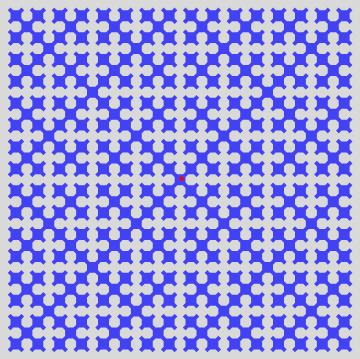
\includegraphics[scale=0.5]{serpinsky.jpg} \end{center}
\caption{Exemple de courbe de Jordan, la courbe de Serpinsky. Le point rouge est-il dans la composante connexe bornée ou non bornée?}\label{fig:serpinsky}
\end{figure}

Une autre façon de décrire un domaine $n$-connexe est la notion de coupures c'est-à-dire une chemin à l'intérieur du domaine reliant les bords de $\Omega$ (cf. figure~\ref{fig:Riemann}). Un domaine borné dans lequel il est possible de trouver $(n-1)$ coupures sans séparer le domaine en deux ou plusieurs composantes connexes sera $n$-connexe. Nous voyons aussi que tout domaine borné $n$-connexe se transforme en un domaine simplement connexe par $(n-1)$ coupures (imaginer le domaine sur tracé sur une feuille de papier dans lequel effectue des découpes au ciseau le long des coupures).

\begin{figure}[ht]
 \begin{center}
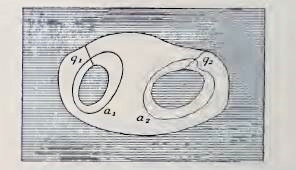
\includegraphics[scale=1]{3_connected_RiemannBis}\hspace*{0.2cm}\end{center}
\caption{Coupures $q_1$, $q_2$ dans un domaine $3$-connexe : image extraite des mathématiques de Riemann.}\label{fig:Riemann}
\end{figure}

Nous observons également dans la figure~\ref{fig:Riemann} que l'adjonction des courbes $a_1$ et $a_2$ forme un encadrement complet du domaine.

La proposition suivante, qui découle du fait qu'un homéomorphisme préserve les classes d'homotopie, montre que le groupe fondamental est caractéristique de la topologie d'un domaine.
\begin{fprop}
Deux domaines homéomorphes ont des groupes fondamentaux isomorphes. En particulier, si l'un est $n$-connexe, l'autre l'est aussi.
\end{fprop}


%La preuve de ce théorème, qui est essentiellement une application de la formule
%de Stokes, va être détaillée à l'aide de deux lemmes fondamentaux.
%\begin{lemma}
%Soit $\gamma \colon [0,1] \to \mathbb{C}$ un lacet simple régulier de
%classe $C^1$. Il existe un nombre fini de couples $(U_i, \theta_i)_{i=1\dots N}$ avec $U_i$
%ouvert de $\mathbb{R}^2$ et $\theta_i$ difféomorphisme de classe $C^1$ de $U_i$
%dans $\mathbb{R}^2$ vérifiant les assertions suivantes:
%\begin{enumerate}
%  \item la famille $(U_i)_{i=1\dots N}$ forme un recouvrement ouvert de l'image
%  de $\gamma$.
%  \item l'image de $\gamma([0,1])\cap U_i$ par $\theta_i$ est un segment de
%  l'axe des abscisses.
%\end{enumerate}
%\end{lemma}
%\begin{proof}
%Soit $\gamma(t_0)$ un point de l'image de $\gamma$. On a, par régularité de
%$\gamma$,  $\gamma^\prime(t_0) \neq 0$. 
%Soit l'application:
%\[
%(t,s) \to \gamma(t) + s v
%\]
%définie pour $t$ assez proche de $t_0$. Sa dérivée en $(t_0,0)$ a pour matrice
%jacobienne:
%\[
%\left(
%\gamma^\prime(t_0), v
%\right)
%\]
%qui est inversible. Le théorème d'inversion locale montre alors qu'il existe un
%voisinage ouvert $U_{t_0}$ contenant $\gamma(t_0)$ et un difféomorphisme
%$\theta_{t_0}$ de classe $C^1$ défini sur $U$ tel que $\theta_{t_0}(U_{t_0})$
%contienne un pavé $]t_0-\epsilon, t_0+\epsilon[ \times ]-\eta, \eta[$ avec
%$\epsilon >0, \eta > 0$. Pour tout $t \in ]t_0-\epsilon, t_0+\epsilon[$, on a
%$\theta^{-1}(t,0)=\gamma(t)$ par construction. En revanche, il peut exister des
%couples $(t,s), s \neq 0$ tels que $\theta^{-1}(t,s)=\gamma(\tilde{t})$, et dans
%ce cas $\tilde{t} \notin ]t_0-\epsilon, t_0+\epsilon[$. Soit $\Delta$ l'ensemble
%de ces couples. Il existe un pavé $]t_0-\epsilon_1, t_0+\epsilon_1[ \times
%]-\eta_1, \eta_1[$ avec $\epsilon_1 > 0$, $\eta_1 > 0$ et ne rencontrant pas
%$\Delta$. Supposons cette propriété fausse. Il existe alors une suite de points
%$(t_i,s_i)$, $s_i \neq 0$ de limite $(t_0,0)$. Pour tout entier $i$, soit
%$\tilde{t}_i$ un point tel que $\gamma(\tilde{t}_i)=\theta^{-1}(t_i,s_i)$. La
%suite $\tilde{t}_i, i\in \mathbb{N}$ appartient au compact $[0,1]$ et admet un point
%d'accumulation $\tilde{t} \notin ]t_0-\epsilon, t_0+\epsilon[$. Par continuité
%de $\gamma$, $\gamma(\tilde{t})=\gamma(t_0)$, ce qui contredit le fait que
%$\gamma$ soit un homéomorphisme. On peut donc choisir l'ouvert $U_{t_0}$ de
%telle sorte que l'image de $\gamma([0,1]\cap U_{t_0})$ soit un segment de l'axe
%des abscisses.
%La preuve du lemme se déduit directement de cette propriéte et de la compacité
%de $\gamma([0,1])$: La famille $(U_t)$ forme un recouvrement ouvert de
%$\gamma([0,1])$, on peut donc en extraire une sous-famille finie qui répond aux
%conditions du lemme.
%\end{proof}
%% Ce lemme permet d'obtenir une forme affaiblie de théorème de Jordan.
%%Pour ce faire, on va montrer qu'il existe une partition de $\mathbb{R}^2$ en points
%%d'indice nul et points d'indice égal à $\pm 1$ (le signe étant toujours le
%%même). On se donne une courbe de Jordan régulière $\gamma$ de classe $C^1$.
%%Soit $x \in \mathbb{R}^2$ et soit $v$ un vecteur quelconque non nul. Si la
%%demi-droite de sommet $x$ et de vecteur directeur $v$ a une intersection vide
%%avec l'image de $\gamma$, l'indice de $x$ est 0: en effet, les points de la
%%demi-droite suffisamment loin de l'origine sont d'indice nul et par continuité
%%de l'indice, $x$ doit aussi avoir un indice nul. Sinon, il existe un nombre fini
%%de domaines $u_i$ dans lesquels une intersection a lieu. En modifiant
%%éventuellement $v$, il est toujours possible de supposer que les intersections 
%%sont réduites à un point. On raisonne de la façon suivante: en partant d'un
%%point de la demi-droite d'indice 0, on chemine vers $x$ (i.e. selon la
%%direction $-v$) jusqu'au premier point d'intersection $x_1$. Après
%%transformation par le difféomorphisme $\theta_1$ correspondant à l'ouvert $U_1$
%%contenant $x_1$, on compare le sens de parcours du chemin et celui du parcours
%%de la demi-droite. Si les deux vecteurs sont en sens direct, on augmente d'une
%%unité l'indice des points placés après l'intersection, sinon on le diminue d'une
%%unité. Cette procédure est schématisée figure \ref{fig:jordan} et s'explique très
%%facilement: dans un cas le chemin s'enroule en sens trigonométrique autour des points situés
%%après l'intersection, l'indice doit donc augmenter, dans l'autre cas il doit
%%diminuer. On répète l'opération de proche en proche jusqu'à atteindre le point
%%$x$. Trois cas uniquement peuvent se présenter: l'index de $x$ vaut $0$
%% s'il y a eu un nombre pair d'intersections, et $+1$ ou $-1$ s'il y en a eu un
%% nombre impair (les signes aux intersections doivent en effet s'alterner, sans
%% quoi on ne pourrait avoir un lacet simple). Pour la même raison, il n'est pas
%% possible d'avoir à la fois des points d'indice $+1$ et $-1$. L'ensemble des
%% points d'indice non nul forme un domaine de $\mathbb{R}^2$, de bord l'image de
%% $\gamma$ et ceux d'indice nul un domaine non borné, ce qui est précisément la
%% conclusion du théorème de Jordan.
%% \begin{figure}[ht]
%%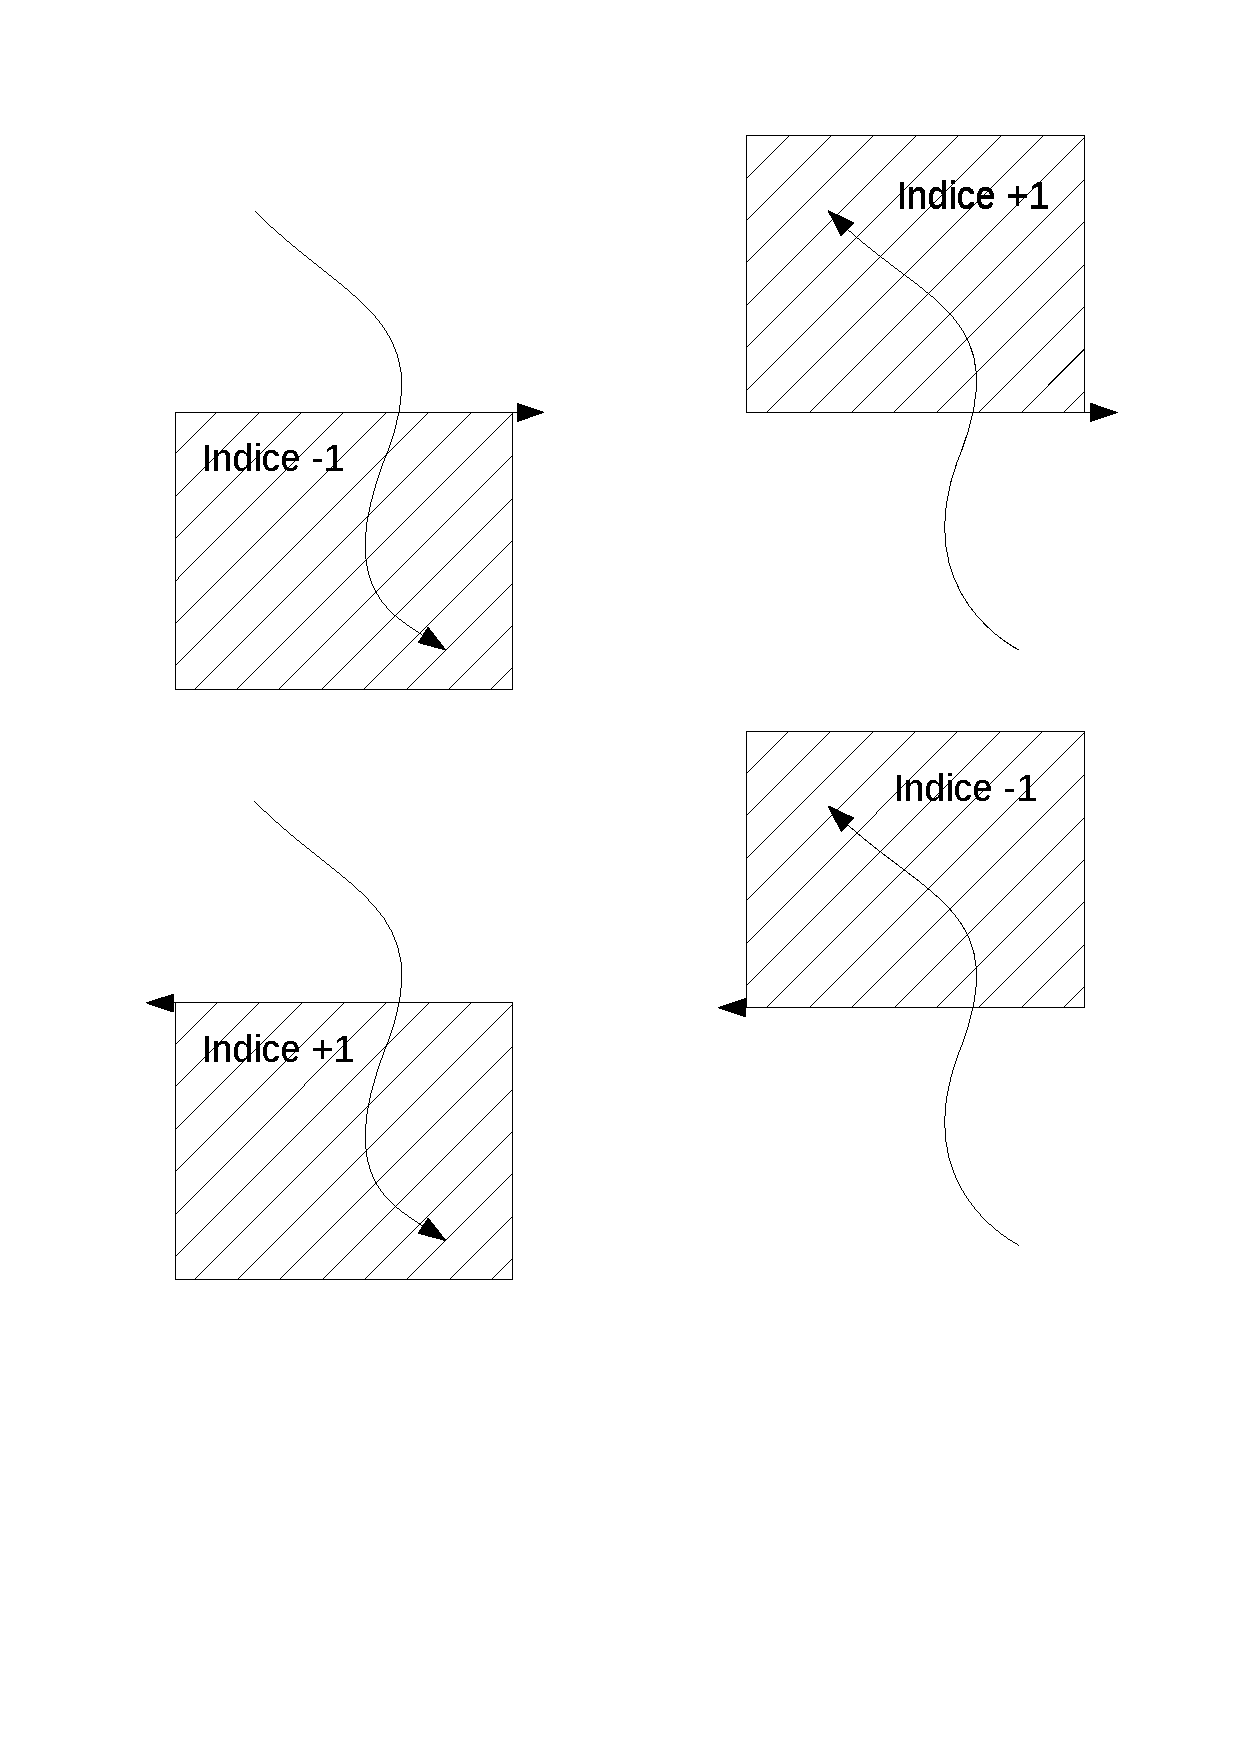
\includegraphics[scale=0.3]{images/jordan.pdf}
%%\caption{Franchissement d'un lacet}\label{fig:jordan}
%%\end{figure}
%%On peut utiliser de façon pratique le procédé précédent pour déterminer
%%rapidement si un point appartient au domaine intérieur à une courbe de Jordan;
%%c'est un algorithme que l'on rencontre couramment dans les logiciels de dessin
%%ou de conception assistée par ordinateur, en concurrence avec celui basé sur un
%%calcul de l'indice par intégration que nous verrons plus loin.
%%
%%On notera la latitude laissée dans le choix de la direction $v$ utilisée dans
%%la preuve du lemme. En particulier, si $U$ est le domaine intérieur à $\gamma$,
%%on pourra toujours choisir les difféomorphismes $\theta_i$ de telle façon 
%%que l'image de  $U \cap U_i$ par $\theta_i^{-1}$ soit contenue dans le
%%demi-espace $\mathbb{R}\times \mathbb{R}^+$. La portion de courbe $\gamma$,
%%forme un segment de l'axe des abscisses et sera parcouru soit dans le sens des 
%%abscisses croissantes, soit dans le sens des abscisses décroissantes. 
%%Dans le premier cas, l'indice devra être +1 pour les points intérieurs
%%et donc -1 dans le second cas. 
%%L'indice étant constant, on en déduit que le sens de parcours sera le même dans
%%tous les morceaux obtenus par applications des $\theta_i^{-1}$. On dira que $\gamma$ est
%%orientée en sens positif si l'indice des points intérieurs est +1, en sens
%%négatif s'il vaut -1. L'orientation d'une courbe de Jordan est toujours
%%possible, mais ceci ne reste plus vrai en dimension supérieure, même pour des
%%surfaces très régulières: des exemples de surfaces $C^\infty$ non orientables
%%peuvent facilement être obtenus.
%
%Le lemme peut être étendu à un chemin de classe $C^1$ par morceaux:
%\begin{lemma}
%Soit $\gamma$ un lacet simple régulier de classe $C^1$ par morceaux. Il
%existe pour tout point $t_0$ où la dérivée de $\gamma$ est discontinue un voisinage ouvert
%$U$ de $\gamma(t_0)$ dans $\mathbb{C}$,un voisinage ouvert $V$ de $(t_0,0)$ dans
%$\mathbb{R}^2$ et un difféomorphisme $\theta$ de classe $C^1$ de $U$ dans $V$
%tels que l'image de $\gamma([0,1]) \cap U$ soit la réunion d'un segment du
%demi-axe des abscisses négatif et d'un segment de l'axe du demi-axe des
%ordonnées positif.
%\end{lemma}
%\begin{proof}
%La démonstration est semblable à celle du lemme précédent. On notera $\gamma^-$
%(resp. $\gamma^+$) la portion de l'image du lacet $\gamma$ formée des points
%$\gamma(t), t < t_0$ (resp. $\gamma(t),t > t_0$). On peut compléter $\gamma^+,
%\gamma^-$ dans un voisinage de $t_0$ de telle façon que le chemin ainsi obtenu
%soit de classe $C^1$:on peut par exemple prolonger par un segment de droite de
%vecteur directeur la limite à gauche (resp. à droite) de la dérivée de $\gamma$
%en $t_0$. On continuera à désigner $\gamma^+, \gamma^-$ les chemins ainsi
%prolongés. Dans un voisinage de $(t_0,t_0)$, on définit l'application:
%\[
%(t,s) \mapsto \gamma(t) + \gamma(s) - \gamma(t_0)
%\]
%Sa matrice Jacobienne en $(t_0,t_0)$ est:
%\[
%\left(
%\gamma^\prime(t_0^-), \gamma^\prime(t_0^+) 
%\right )
%\]
%qui est de rang maximal si $t_0$ est un point de discontinuité de la dérivée. 
%Le théorème d'inversion locale permet alors de conclure.
%\end{proof}
% Il est maintenant possible de procéder à la preuve du
%théorème.
%\begin{proof}
%On posera $f = P + i Q$. Soit $U$ le domaine intérieur bordé par le lacet simple régulier $\partial \Omega$. Soient enfin $U_i, i=1\dots N$ les ouverts
%donnés par le premier ou le second lemme selon que l'on est ou non au voisinage
%d'un point de discontinuité de la dérivée. Le recouvrement ouvert $U \cup
%\bigcup_{i=1}^N U_i$ admet une partition de l'unité $\alpha_i, i=0\dots N$ subordonnée 
%(on note $\alpha_0$ le terme associé à $U$). Considérons les formes différentielles continues de
%degré 1:
%\[
%\omega_1 = P dx - Q dy, \quad \omega_2= Qdx + Pdy 
%\]
%on a:
%\[
%d\omega_1 = -\left(\frac{\partial P}{\partial y}+\frac{\partial Q}{\partial
%x}\right )dx \wedge dy
%\]
%et
%\[
%d\omega_2 = \left(\frac{\partial P}{\partial x}-\frac{\partial Q}{\partial
%y}\right )dx \wedge dy
%\]
%L'intégrale:
%\[
%\int_{U} \alpha_0 d\omega_1 = - \int_{U}\alpha_0(x,y) \left(\frac{\partial
%P}{\partial y}(x,y)+\frac{\partial Q}{\partial x}(x,y)\right )dxdy
%\]
%vaut $0$, le support de $\alpha_0$ se trouvant dans $U$. La même propriété
%est vraie pour $d\omega_2$. Soit maintenant un des ouverts $U_i, i=1\dots N$ et
%$\theta_i^{-1}$ le difféomorphisme de classe $C^1$ associé (on choisit de
%travailler avec $\theta_i^{-1}$ pour simplifier les notations). On remarquera
%tout d'abord (le vérifier !) que $\theta_i^*\left(\alpha_i d \omega_1\right) =
%\alpha_i\circ \theta_i d \theta_i^* \omega_1$. On a donc:
%\[
%\int_{U_i} \alpha_i d \omega_1  = \int_{\theta_i(U_i)} \alpha_i\circ \theta_i d
%\theta_i^* \omega_1
%\]
%La formule de Stokes élémentaire (qui s'étend très facilement dans le
%cas des images d'ouverts contenant une singularité) appliquée à l'ouvert
%$\theta_i(U_i)$ montre que l'intégrale précédente vaut $\int_{\theta_i(\gamma[0,1]\cap U_i)} 
%\left (\alpha_i \circ \theta_i\right) \theta_i^*(\omega_i)$ qui s'identifie à
%l'intégrale de la partie réelle de $f$ sur la portion de chemin appartenant à
%$U_i$. Un raisonnement similaire peut se faire sur $\omega_2$: on en déduit le
%théorème par sommation sur les $U_i$.
%\end{proof}


%  le domaine par des coupures et des ch n'est pas valable pour des domaines présentant des trous, tels celui de la figure \ref{fig:domaine_trois_connexe}.
%\begin{figure}[ht]
%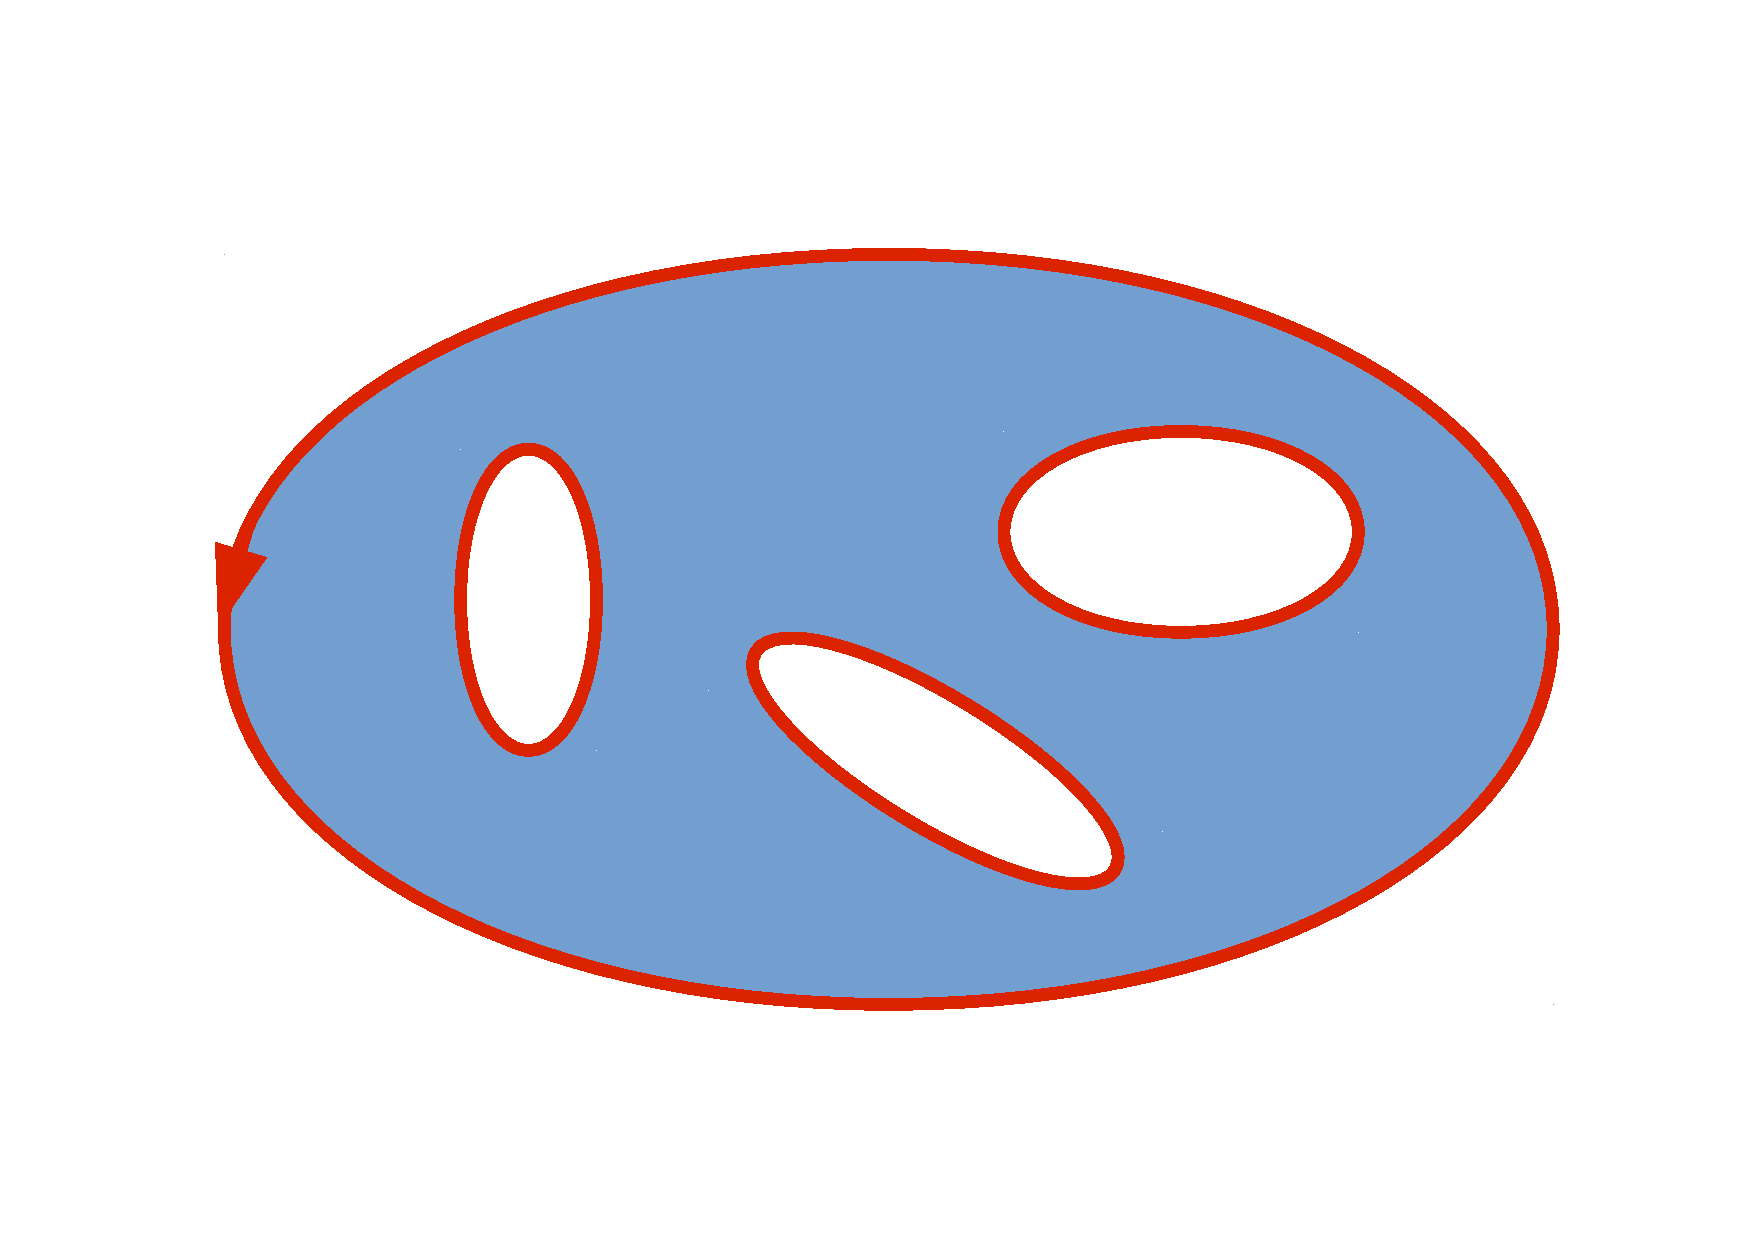
\includegraphics[scale=0.3]{images/domaine_trois_connexe.pdf}
%\caption{Domaine 3-connexe}\label{fig:domaine_trois_connexe}
%\end{figure}
%Si le bord est formé d'une union disjointe de lacets simples réguliers de classe $C^1$, on peut néanmoins continuer à appliquer le théorème en prenant garde à orienter en sens direct le contour extérieur et en sens rétrograde les lacets internes. 

%\begin{figure}[H]
%\begin{center}
%\shorthandoff{!}\shorthandoff{:}
%\begin{tikzpicture}
%\tikzset{
%    on each segment/.style={
%        decorate,
%        decoration={
%            show path construction,
%            moveto code={},
%            lineto code={
%                \path [#1]
%                (\tikzinputsegmentfirst) -- (\tikzinputsegmentlast);
%            },
%            curveto code={
%                \path [#1] (\tikzinputsegmentfirst)
%                .. controls
%                (\tikzinputsegmentsupporta) and (\tikzinputsegmentsupportb)
%                ..
%                (\tikzinputsegmentlast);
%            },
%            closepath code={
%                \path [#1]
%                (\tikzinputsegmentfirst) -- (\tikzinputsegmentlast);
%            },
%        },
%    },
%     mid arrow/.style={postaction={decorate,decoration={
%        markings,
%        mark=at position .5 with {\arrow[#1]{stealth}}
%      }}},
%}
%    
%
%    \begin{scope}[scale=4]
%        \draw[pblue, fill=gray!60] plot [smooth,tension=1]
%        coordinates {(0,0)  (0.5,-0.5) (1.5,-0.25) (1.5,0.25)  (0.5,0.5)    (0,0)}[postaction={on each segment={draw,-{latex[red]}}}];
%        \draw[pblue, fill=white] (0.5,0) circle(0.1)[postaction={on each segment={draw,-{latex[red]}}}];
%        \draw[pblue, fill=white,postaction={on each segment={mid arrow=red}}] (1,0.2) circle(0.15);
%     
% 
%   \end{scope}        
%\end{tikzpicture}
%
%\shorthandon{!}\shorthandoff{:}
%
%\end{center}
%\end{figure}

%\begin{figure}[H]
%\begin{center}
%\shorthandoff{!}\shorthandoff{:}
%\begin{tikzpicture}[line cap=round,line join=round,>=triangle 45,x=1.0cm,y=1.0cm, scale=0.5]

% \clip(0,-8) rectangle (15,5);
% \draw [rotate around={-0.1578392137018885:(7.63,-2.01)},line width=1.2pt,color=pblue,fill=gray!60] (7.63,-2.01) ellipse (6.0030616253714175cm and 4.781186973755255cm);
% \draw [->,line width=1.2pt,color=red] (4.843684536671036,2.2277812530546623) -- (3.7161360857926025,1.6192210028084606);
% \draw [rotate around={34.28687697720894:(5.3,-3.08)},line width=1.2pt,color=pblue, fill=white] (5.3,-3.08) ellipse (1.6499992990844683cm and 1.260197479357598cm);
% \draw [rotate around={-37.647620640107654:(10.05,0.19)},line width=1.2pt,pblue, fill=white] (10.05,0.19) ellipse (1.520903173802141cm and 0.7446787656979887cm);
% \draw [->,line width=1.2pt,color=red] (2.3544469454010093,0.2767507959517612) -- (4.452721092020469,-2.1406480215607453);
% \draw [->,line width=1.2pt,color=red] (6.590412502340801,-3.5265753913741547) -- (6.1495589441687315,-4.017514015411874);
% \draw [->,line width=1.2pt,color=red] (4.210387657702547,-2.369374149876248) -- (2.18,0.);
% \draw [->,line width=1.2pt,color=red] (5.574171034883071,-6.500008723492629) -- (6.86501766619565,-6.751443315622627);
% \draw [->,line width=1.2pt,color=red] (12.437764207761877,-4.877899122285109) -- (13.06827265799081,-4.04009189652059);
% \draw [->,line width=1.2pt,color=red] (10.976430622084985,1.956011041629362) -- (10.223489836526179,0.9727657697766641);
% \draw [->,line width=1.2pt,color=red] (9.950092242322414,1.1184639373638194) -- (10.698285458294508,2.0963876646929642);
% \draw [->,line width=1.2pt,color=red] (9.967860540261333,-0.6458868355720401) -- (9.33023650232943,-0.17002180107179365);
% \end{tikzpicture}
% \shorthandon{!}\shorthandoff{:}
% \caption{Chemin d'intégration dans un domaine $3$-connexe, expliquant les orientations choisies sur les bords.}
% \end{center}
% \end{figure}



% \begin{figure}[ht]
%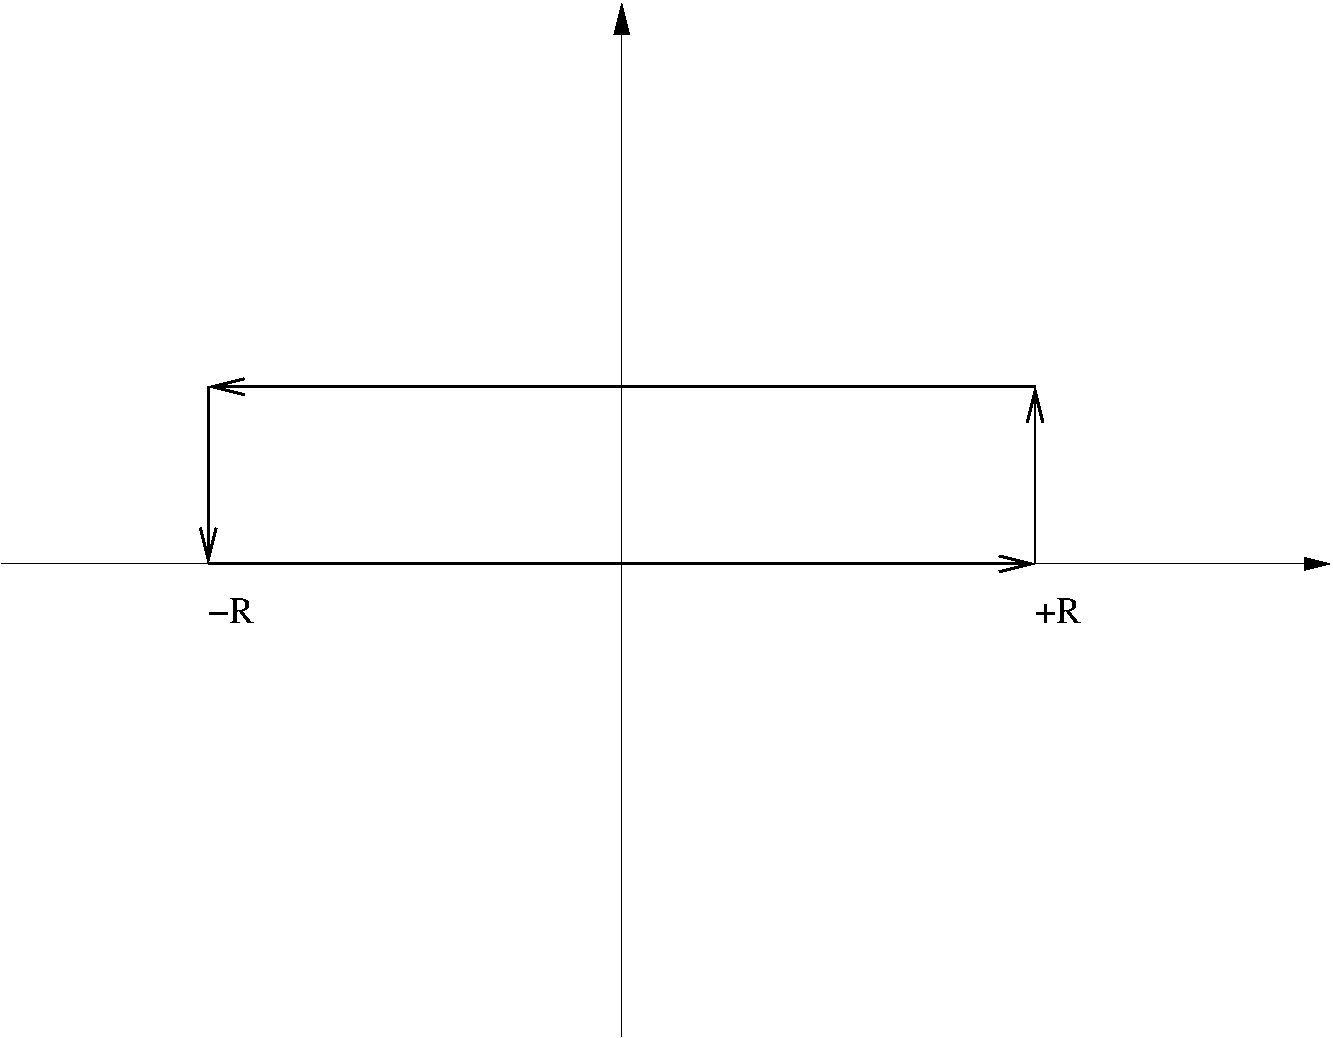
\includegraphics[scale=0.3]{images/contour_gauss.pdf}
%\caption{Contour $\gamma_r$}\label{fig:contour3}
%\end{figure}


\subsection{Théorème de Goursat}
 Nous avons vu précédemment que si une application continue définie sur un ouvert admet une primitive, son intégrale le long d'un chemin de classe $C^1$ est simple à calculer. Il est donc important de disposer d'un critère premettant de savoir si l'on se trouve dans ce cas.

En général une fonction, même analytique dans un domaine $\Omega$ n'admet pas nécessairement de primitive dans $\Omega$, par ex. la fonction $1/z$ dans le disque unité privé de l'origine. Cependant, si la série entière 
\[f(z)=a_0 + a_1 (z-z_0) +\cdots + a_n (z-z_0)^n + \cdots\]
est convergente dans le disque $\lvert z-z_0 \rvert <r$, alors la série entière
\[F(z)=a_0 (z-z_0) + \frac{a_1}{2} (z-z_0)^2 +\cdots + \frac{a_n}{n+1} (z-z_0)^{n+1} + \cdots\]
est convergente dans ce disque et $F$ y est une primitive de $f$.

Nous allons maintenant énoncer une condition suffisante pour l'existence d'une primitive locale. 

\begin{fdefn}
Le triangle $T(z_0,z_1, z_2)$ de sommets $z_0,z_1,z_2$ est l'ensemble des points $\lambda_0 z_0 + \lambda_1 z_1 + \lambda_2 z_2$ avec $\lambda_i \in [0,1]$, $i=1,2,3$ et $\lambda_0 + \lambda_1 + \lambda_2 =1$. Son bord $\partial T$ est appelé lacet triangulaire de sommets $z_0,z_1,z_2$, c'est un lacet simple de
classe $C^1$ par morceaux. Ce lacet s'obtient en considérant les points du triangle pour lesquels l'un des $\lambda_i=0$.
\end{fdefn}

Ce type de chemins joue un rôle particulier en théorie de l'intégration. La
propriété suivante est simple, mais fondamentale.

\begin{fthm}(Morera)
Soit $\Omega$ un domaine de $\mathbb{C}$ et $f \colon \Omega \to \mathbb{C}$ une
application continue. Si l'intégrale de $f$ le long de tout lacet triangulaire
de $\Omega$ est nulle, alors au voisinage de tout point $z_0 \in \Omega$, il
existe une application holomorphe $F$ de dérivée égale à $f$. $F$ est appelée \textbf{primitive locale}.
\end{fthm}

\begin{proof}
Soit $z_0 \in \Omega$ et soit $D_{z_0}$ un disque ouvert centré en $z_0$ et
contenu dans $\Omega$. Pour tout $z \in D_{z_0}$, on désigne par $[z_0 ; z]$ le segment reliant $z_0$ à $z$ (chemin $\gamma(t)=z_0 + t(z-z_0)$), et on définit la fonction $F$ par
\[ F(z) = \int_{[z_0 ; z]} f(w) \diff w.
\]
\begin{figure}[ht]
 \begin{center}
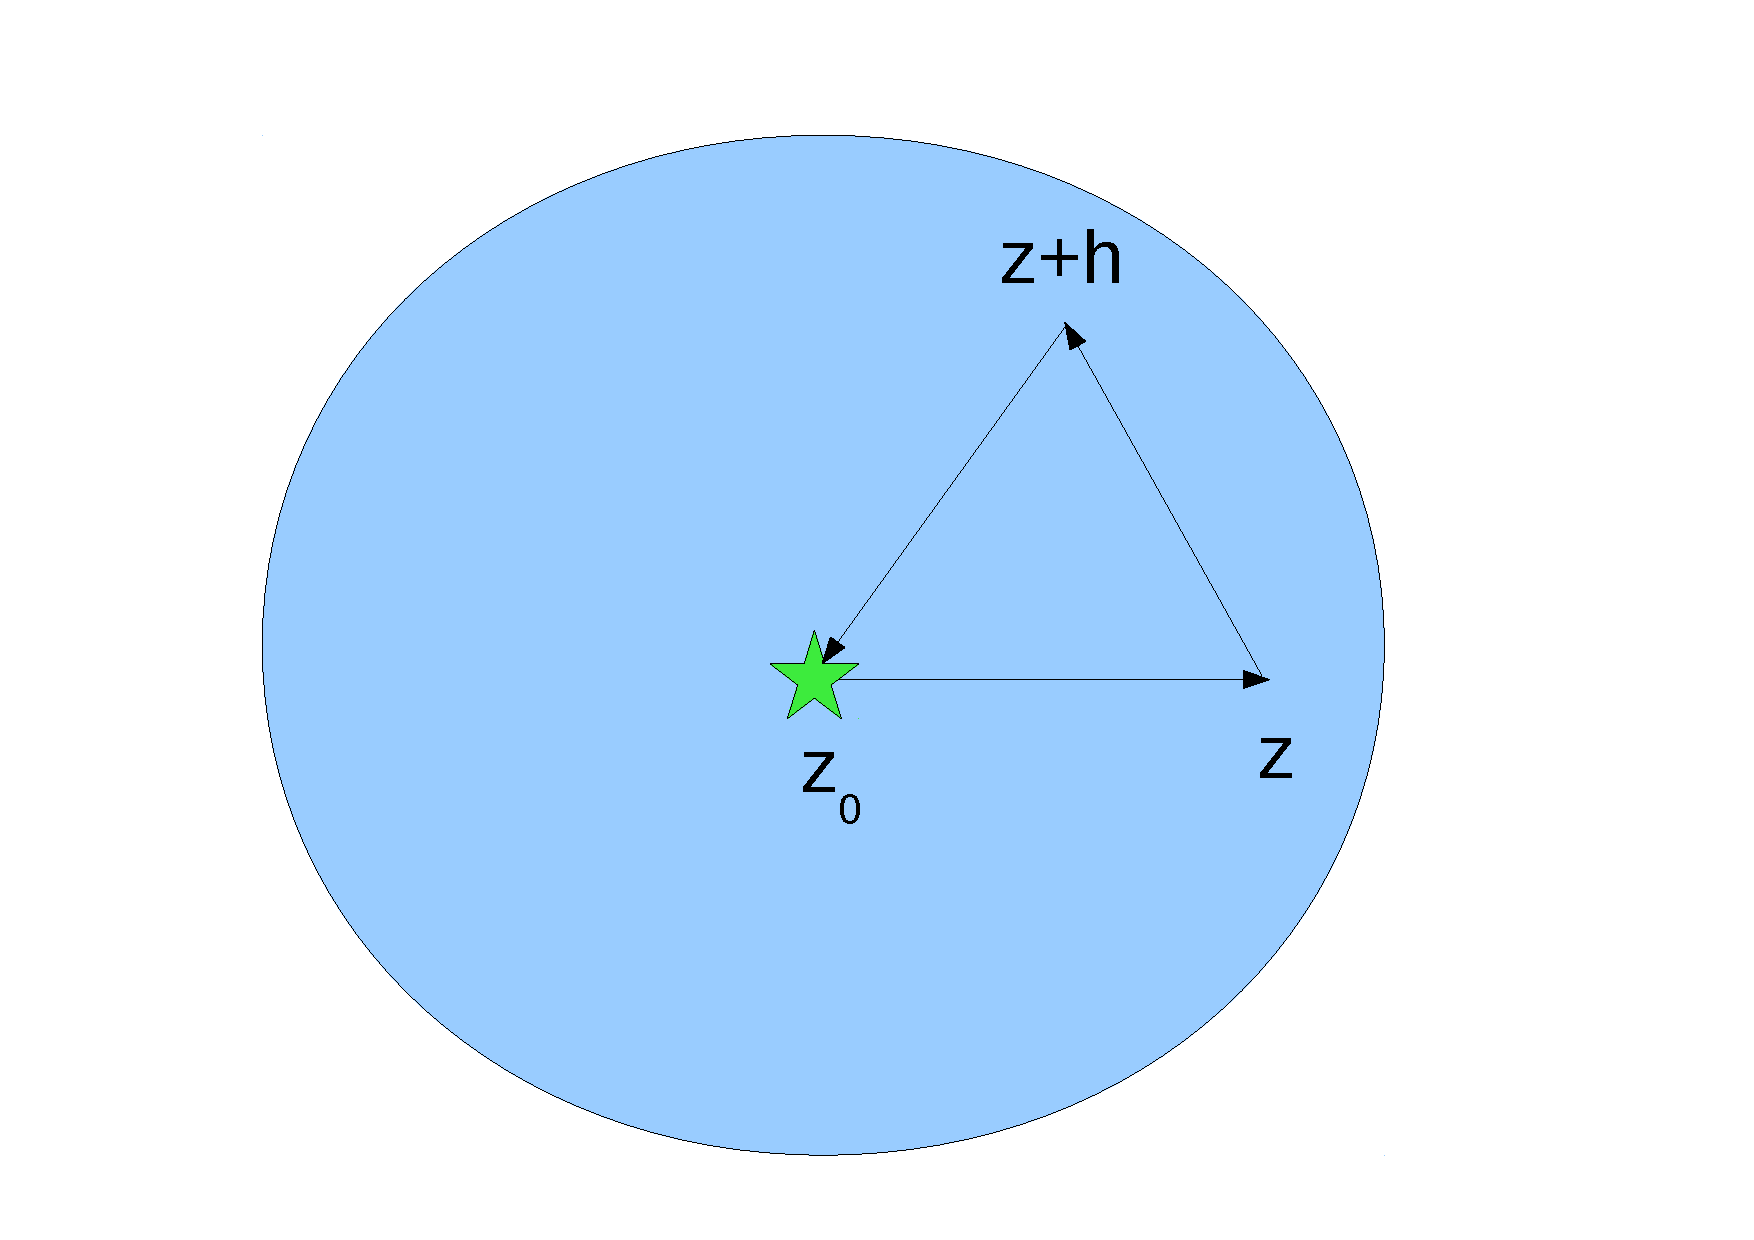
\includegraphics[scale=0.3]{images/morera.pdf}
\caption{Lacet triangulaire}\label{fig:morera}
\end{center}
\end{figure}
Soit $z \in D_{z_0}$ et soit $h \in \mathbb{C}$ tel que
$z+h \in D_{z_0}$. On considère le lacet triangulaire de sommets $z_0,z,z+h$ (cf. figure~\ref{fig:morera}) inclus dans $D_{z_0}$ et on obtient par hypothèse que~:
%\[F(z) + \int_{[z ; z+h]} f(\omega) \diff \omega - F(z+h)=0,\]
%d'où
\[F(z+h)-F(z) = \int_{[z ; z+h]} f(w) \diff w.\]
Puisque $z$ est fixé, la valeur $f(z)$ est constante, d'où
\[F(z+h)-F(z) - h f(z)= \int_{[z ; z+h]} (f(w)-f(z)) \diff w.\]
En divisant par $h$ et en utilisant l'inégalité ML, nous obtenons
\[ \left \lvert \frac{F(z+h)-F(z)}{h} - f(z)\right\rvert \leq M_\epsilon, \quad h<\epsilon \]
où $M_\epsilon$ est le maximum de $\lvert f(w)-f(z)\rvert$ pour tout $w$ tel que $\lvert z -w \rvert <\epsilon$.
Par continuité de $f(w)$ en $z$, $M_\epsilon$ tend vers $0$, lorsque $\epsilon \to 0$, d'où $F(z)$ est holomorphe, et $F'(z)=f(z)$. Ceci est vérifié en tout point de
$D_{z_0}$. 
\end{proof}
% \begin{figure}[ht]
% \begin{center}
%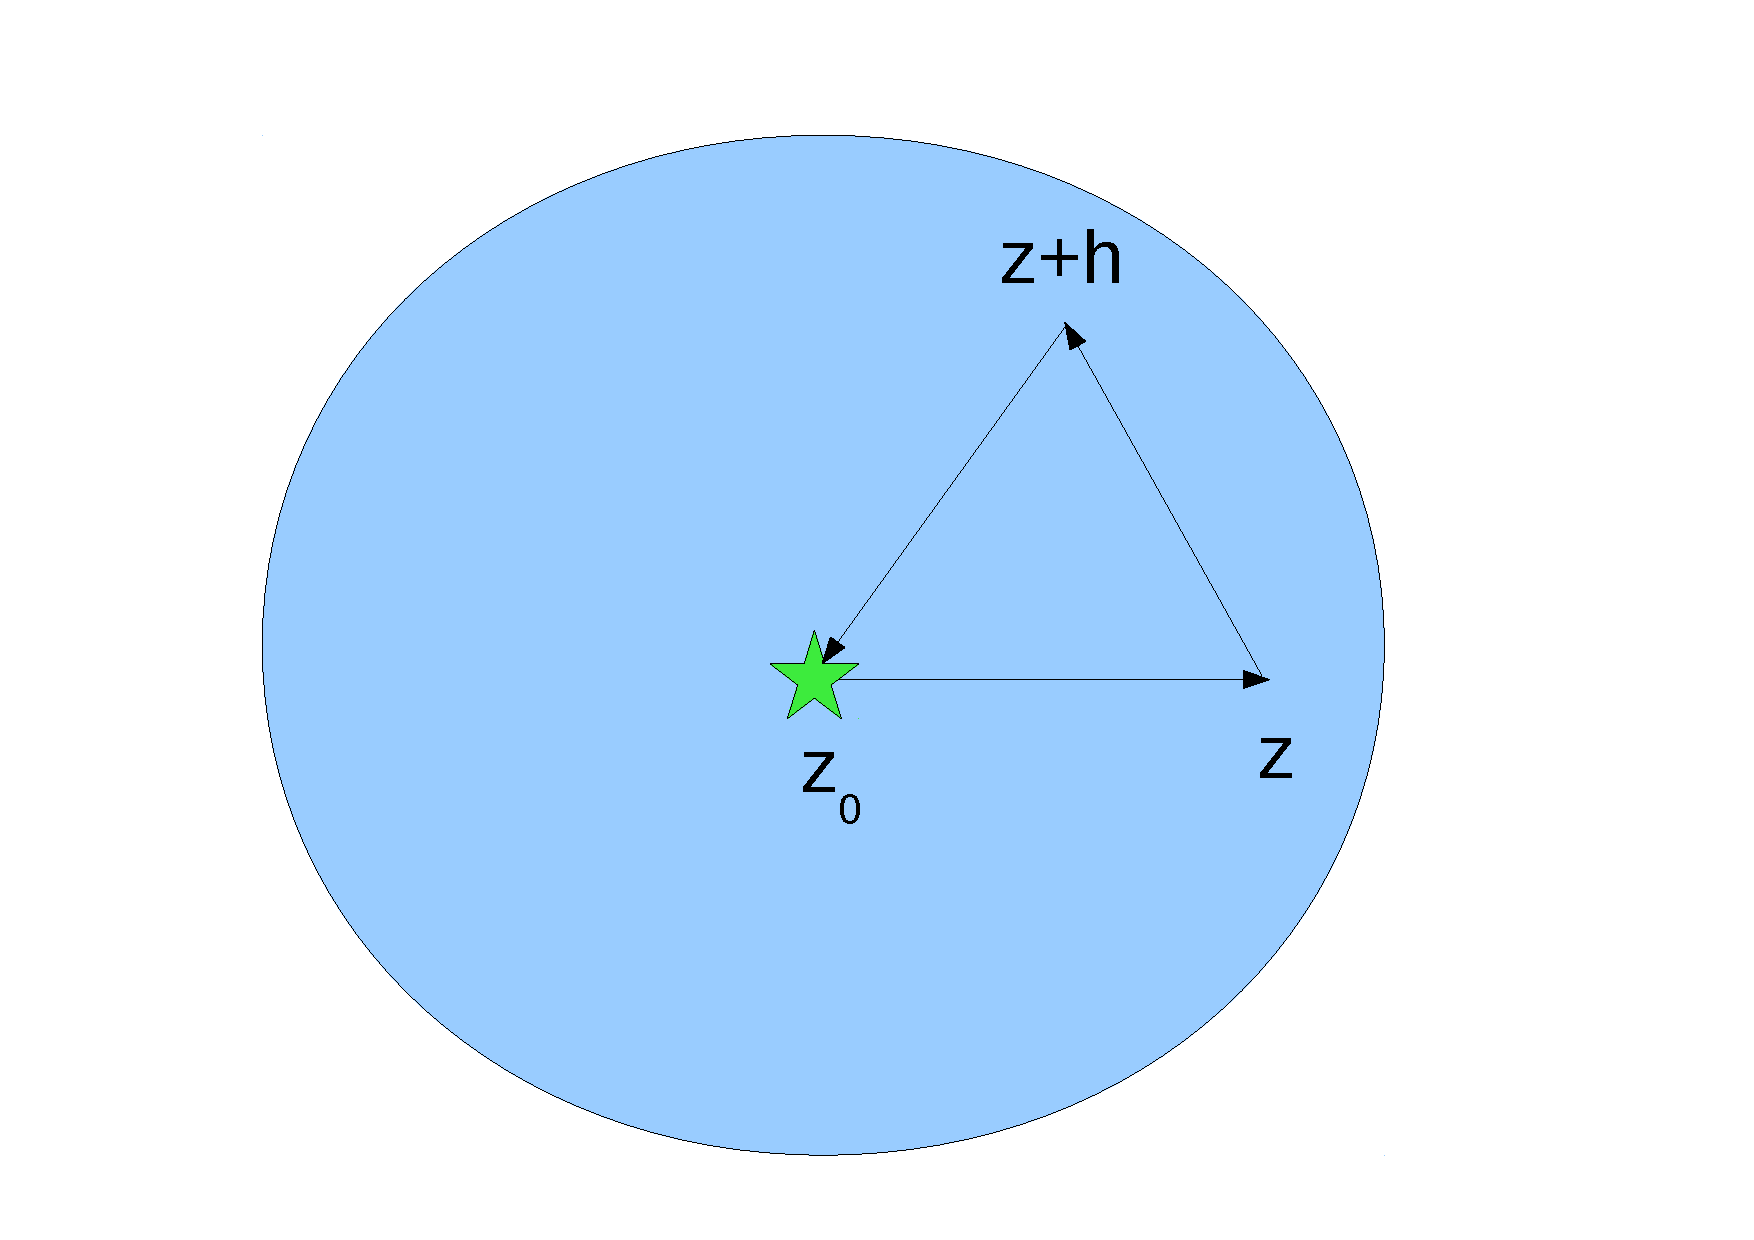
\includegraphics[scale=0.3]{images/morera.pdf}
%\caption{Lacet triangulaire}\label{fig:morera}
%\end{center}
%\end{figure}
On notera que si $F$ est une primitive locale, il en est de même pour $F+c$ où
$c$ est un complexe quelconque.

On souhaite maintenant définir une primitive globale le long d'un chemin $\gamma$. L'idée est de recouvrir l'image du chemin dans $\C$ (qui est compact) par un nombre fini de disques dans chacun desquels existera une primitive locale. Il suffira alors de recoller ces primitives locales pour définir une primitive globale. 

\begin{fprop}(Primitive le long d'un chemin)
\label{prop:primitive_chemin}
Soit $\Omega$ un \textbf{domaine} de $\mathbb{C}$ et soit $f$ vérifiant les hypothèses
de la proposition précédente. Soit $\gamma$ un chemin de $\Omega$. Il existe
alors une application continue $\theta_\gamma \colon [0,1] \to \mathbb{C}$ telle 
que pour tout $t \in [0,1]$, il existe un voisinage $V_t$ de $\gamma(t)$
dans $\Omega$, une application $F_t$, holomorphe de classe $C^1$ sur $V_t$, de
dérivée égale à $f$ et vérifiant $\theta_\gamma(u)=F_t(\gamma(u))$ au voisinage de $t$. La fonction $\theta_\gamma$ est appelée primitive de $f$ le long de $\gamma$ et on aura
\[\int_{\gamma} f(z) \diff z = \theta_\gamma(1)-\theta_\gamma(0).\]
\end{fprop}

\begin{proof}
On va montrer par un procédé constructif la possibilité d'obtenir $\theta_\gamma$. L'image de $\gamma$ est
un compact, on peut donc la recouvrir par un nombre fini de disques ouverts
$D_i, i=1\dots N$ sur lesquels on peut obtenir, par la proposition
précédente, une primitive $F_i$ de $f$. Sur $D_i \cap D_{i+1}$, on a $\left(F_{i+1}(z) -F_i(z)\right)^\prime=f(z)-f(z)=0$, donc par connexité, $F_{i+1} = F_i +c$, avec $c$ une constante que l'on peut choisir égale à $0$. 


 
\begin{figure}[ht]
\begin{center}
\shorthandoff{!}\shorthandoff{:}
\begin{tikzpicture}
\tikzset{
    on each segment/.style={
        decorate,
        decoration={
            show path construction,
            moveto code={},
            lineto code={
                \path [#1]
                (\tikzinputsegmentfirst) -- (\tikzinputsegmentlast);
            },
            curveto code={
                \path [#1] (\tikzinputsegmentfirst)
                .. controls
                (\tikzinputsegmentsupporta) and (\tikzinputsegmentsupportb)
                ..
                (\tikzinputsegmentlast);
            },
            closepath code={
                \path [#1]
                (\tikzinputsegmentfirst) -- (\tikzinputsegmentlast);
            },
        },
    },
}
    
\begin{scope}[scale=2]
        \node (A) at (0,0) {};
        \node (B) at (2,0.25){};
        \draw[blue] plot [smooth,tension=1]
        coordinates {(A) (0.5,0.5) (1.5,0) (B)}[postaction={on each segment={draw,-{stealth[red,bend]}}}];
       \draw [fill=black] (A) circle (1pt);
    \draw [fill=black] (B) circle (1pt);
\draw  (A) circle(0.3) ;
\draw  (B) circle(0.3) ;
\draw (0.5,0.5) circle(0.3) ; 
\draw (0.25, 0.32) circle(0.3) ; 
\draw (0.85, 0.38) circle(0.3) ; 
\draw (1.2, 0.13) circle(0.3) ; 
\draw (1.6, 0) circle(0.3) ; 



\draw [fill=black] (0.25, 0.32) circle (1pt);
\draw [fill=black] (0.5, 0.5) circle (1pt);
\draw [fill=black] (0.85, 0.38) circle (1pt);
\draw [fill=black] (1.2, 0.13) circle (1pt);
\draw [fill=black] (1.6, 0) circle (1pt);
  \end{scope}    
    
\end{tikzpicture}
\shorthandon{!}\shorthandoff{:}
%\caption{}
\end{center}
\end{figure}
 
Quitte à réordonner la numérotation des boules $D_i$,
on peut obtenir une subdivision $0=t_0 < t_2 < \dots < t_N = 1$ de $[0,1]$
telle que $\gamma([t_{i-1},t_i])\subset D_i, i =1\dots N$. On peut choisir $F_1$ de telle sorte que
$F_1(\gamma(0))=\theta_\gamma(0)$, puis pour $i=2, \cdots, N$, on pose pour $u \in [t_{i-1},t_i]$,
$\theta_\gamma(u)=F_i(\gamma(u))$. La fonction $\theta_\gamma$ ainsi obtenue est bien définie et 
\[\int_{\gamma([t_{i-1}, t_i])} f(z) \diff z = F_i(\gamma(t_i)) - F_i(\gamma(t_{i-1})) = \theta_\gamma(t_i) - \theta_\gamma(t_{i-1}),\]
d'où
\[\int_\gamma f(z) \diff z = \sum_{i=1}^N \left(\theta_\gamma(t_i) - \theta_\gamma(t_{i-1})\right)=\theta_\gamma(1) - \theta_\gamma(0).\]
%Supposons obtenue $\theta$ jusqu'à $t_i$. Sur le domaine $B_i \cap B_{i+1}$, la
%différence entre $F_i,F_{i+1}$ est de dérivée nulle, donc cette différence est
%constante. On peut choisir $F_{i+1}$ de telle sorte qu'elle soit nulle, ce qui
%définit $\theta$ de proche en proche.
\end{proof}

Dans le cas où une application vérifie les hypothèses de la proposition
précédente, l'existence d'une primitive locale $\theta_\gamma$, le long de $\gamma$, permet d'écrire~:
\[
\int_{\gamma} f(z) \diff z = \theta_\gamma(1)-\theta_\gamma(0).
\] 

Cette intégrale dépend du chemin $\gamma$ et en particulier n'est pas nécessairement nulle si le chemin est un lacet. La différence provient de l'impossibilité de satisfaire deux conditions de recollement pour le dernier disque recouvrant $\gamma(0)=\gamma(1)$. On a néanmoins une
invariance par déformation continue du chemin en laissant les extrémités fixées : c'est la notion d'homotopie, très importante pour la suite.


Nous avons vu comment calculer (du moins en théorie) l'intégrale d'une fonction continue et d'intégrale nulle sur tout chemin triangulaire, et nous avons noter que cette intégrale dépend du chemin reliant deux extrémités fixées. L'homotopie apporte un éclairage sur cette dépendance, car nous avons résultat important suivant :

\begin{fthm}(Invariance par homotopie)\label{the:invar}
Soit $\Omega$ un domaine de $\mathbb{C}$ et soient $\gamma_1, \gamma_2$ deux
chemins de $\Omega$, homotopes à extrémités fixées. Soit $f \colon
\Omega \to \mathbb{C}$ continue et dont l'intégrale le long de tout lacet
triangulaire de $\Omega$ s'annule. Alors:
\[
\int_{\gamma_1} f(z) \diff z = \int_{\gamma_2} f(z) \diff z
 \]
\end{fthm}

\begin{proof}
Soit $\gamma_1$ et $\gamma_2$ deux chemins reliant $p$ à $q$ et homotopes dans un domaine $\Omega$. Soit $f \colon \Omega \to \C$ une application continue et d'intégrale nulle le long de tout lacet triangulaire. Alors $f$ admet une primitive locale en tout point. Soit $H$ l'homotopie entre entre $\gamma_1 = H(0,\cdot)$ et $\gamma_2=H(1,\cdot)$ ; l'image par $H$ du carré $[0,1]\times [0,1]$ est un compact de $\Omega$, elle peut donc être recouverte par un nombre fini de disques ouverts $\Delta_{hk}$ dans lesquels la fonction $f$ admet une primitive locale (il suffira de choisir un rayon suffisamment petit). Soit alors un découpage de $[0,1]\times [0,1]$ en carrés $R_{hk}$ de telle façon que $H(R_{hk}) \subset  \Delta_{hk}$ (cf. figure~\ref{fig:proofhomotopy}). Cela revient à trouver deux subdivisions $0=t_0 <t_1\cdots <t_n=1$ et $0=s_0 <s_1\cdots <s_m=1$ telles que $R_{hk} = [s_k,s_{k+1}] \times [t_h, t_{h+1}]$.




% Soit $H$ l'homotopie entre $\gamma_1$ et $\gamma_2$. Pour tout
%point $H(t,s)$, il existe une boule ouverte $B$ centrée sur ce point et contenue
%dans $\Omega$ qui est ouvert. Par continuité de $H$, on en déduit l'existence
%d'un pavé $]t_1,t_2[\times ]s_1,s_2[$ contenant $(t,s)$ et dont l'image est dans
%$B$. La collection de ces pavés forme un recouvrement du compact
%$[0,1]\times[0,1]$, il en existe donc une famille finie $\mathcal{S}$ qui
%constitue aussi un recouvrement. Comme $\mathcal{S}$ est finie, on peut
%construire une subdivision de $[0,1]\times[0,1]$ sous la forme de pavés
%$\Delta_{ij}=[t_i, t_{i+1}]\times [s_j,s_{j+1}], \, i=0\dots N-1, j=0,\dots M-1$
%avec $t_0=s_0=0$, $t_N=s_M=1$ tels que pour tout couple $(i,j)$,
%$H(\Delta_{ij})$ est inclus dans un des membres de la famille $\mathcal{S}$. 
%L'intégrale de $f$ étant nulle le long de tout lacet triangulaire, elle admet
%une primitive dans chacune des boules de la famille $\mathcal{S}$ (reprendre la
%démonstration précédente) et donc l'intégrale de $f$ le long du bord de
%$\Delta_{ij}$ est nulle (différence de la primitive en deux points identiques).
%De proche en proche, on en déduit que l'intégrale de $f$ le long des chemins $s \mapsto
%H(t_i,s)$ est constante, soit finalement que l'intégrale de $f$ le long de
%$\gamma_1$ est égale à celle le long de $\gamma_2$.
%

\begin{figure}[H]
\begin{center}
\shorthandoff{!}\shorthandoff{:}
\begin{tikzpicture}
  [decoration={markings,mark=at position 0.5 with {\arrow{>}}},
   witharrow/.style={postaction={decorate}},
   dot/.style={draw,fill,circle,inner sep=1.5pt,minimum width=0pt}
  ]

  % rectangle
  \begin{scope}[scale=2]
     \draw[thick]
       (0,0) coordinate (a1) -- node[left]     {$p$} (0,2) coordinate (d1)
       (2,0) coordinate (b1) -- node[right](q1){$q$} (2,2) coordinate (c1);
     \draw[xstep=1/3,ystep=1/3] (a1) grid (c1);
     \draw[thick,witharrow, red] (d1) -- node[above]    {$\gamma_2$}(c1);
     \draw[thick,witharrow, pblue] (a1) -- node[below](f1){$\gamma_1$}(b1);
     \draw[thick,witharrow, color=black!60!green] (0,1-1/3) -- node[below](f1){}(2,1-1/3);
     \draw[thick,witharrow, color=magenta] (0,1) -- node[below](f1){}(2,1);
     \draw[pattern=north west lines, pattern color=black!60!green] (1,1-1/3) rectangle (1+1/3,1);
  \end{scope}


  % ellipse
  \begin{scope}[shift={(6,0.5)}, scale=1.5]
    \node[dot,label={[left] $p$}] (a3) at (0,0) {};
    \node[dot,label={[right]$q$}] (b3) at (4,0) {};
    \draw[name path=red,thick,witharrow, red] (a3) to[out=50,in=150]node[above]{$\gamma_2$} (b3);
    \foreach \o/\i in {40/160,30/170,20/180,10/190,-10/200}
       \draw (a3) to[out=\o,in=\i]  (b3);
    \draw[name path=blue,thick,witharrow, pblue] (a3) to[out=-20,in=-130]node[below]{$\gamma_1$} (b3);
    \draw ($0.5*(a3)+0.5*(b3)$) circle[x radius=2.5,y radius=1.5];
    \node at ($(a3)+(0.5,0.8)$) (X3) {$\Omega$};
    \draw[name path=vert, thick,color=black!60!green] (a3) to[out=10,in=190]  (b3) ;
    \draw[name path=magenta,thick,color=magenta] (a3) to[out=20,in=180]  (b3);
  %  \draw (a3)++(0:2) node[red]{$\bullet$};
  \draw[name path=delta] (a3)++(3:2) circle (0.4);
\path[name path=red1] (a3) circle(1.75cm);
\path[name path=red2] (a3) circle(2.25cm);
\fill[name intersections={of=vert and red1, by=u}] (u) ;
 \fill[name intersections={of=vert and red2, by=v}] (v) ; 
 \fill[name intersections={of=blue and red1, by=w}] (w) ;
 \fill[name intersections={of=blue and red2, by=x}] (x) ; 
 \fill[name intersections={of=red and red1, by=y}] (y) ;
 \fill[name intersections={of=red and red2, by=z}] (z) ; 
 \fill[name intersections={of=magenta and red1, by=t}] (t);
 \fill[name intersections={of=magenta and red2, by=s}] (s) ; 

 \draw plot [smooth,tension=1]
        coordinates {(y) (t) (u)  (w)};
\draw plot [smooth,tension=1]
        coordinates {(z) (s) (v)  (x)};

\filldraw[draw=black,pattern=north west lines, pattern color=black!60!green]
plot [smooth,tension=1]
        coordinates {(u)  (v)} plot [smooth,tension=1]
        coordinates {(v)  (s)} -- plot [smooth,tension=1] coordinates {(s) (t)} -- plot [smooth,tension=1] coordinates {(t) (u)};
%  \fill[color=gray]
%  
%  
%  cycle;

\path[name path=arr] (2,-1) -- (t) ;
\fill[name intersections={of=delta and arr, by=d}] (d) ;
\draw (1.5,-1.7) edge[bend right, ->] (d);
\draw (1.5,-1.7) node[below] {$\Delta_{h,k}$};
  \end{scope}

  % connecting arrows
 
  \draw[-stealth,shorten >=4mm] (q1) -- node[above]{$H$} (X3);
\draw (1.5,-1)  edge[bend right, ->]  (2.5,1.3);
\draw (1.7,-1) node[below] {$R_{h,k}$};
 
%
%\draw (1.7,-1) node[below] {$R_{h,k}$};





\end{tikzpicture}
\shorthandon{!}\shorthandoff{:}
\caption{}\label{fig:proofhomotopy}
\end{center}
\end{figure}

Comme $f$ admet une primitive locale dans $\Delta_{hk}$, son intégrale le long du lacet $\gamma_{h,k} + \beta_{h+1,k} - \gamma_{h,k+1}- \beta_{h,k}$ est nulle. Par conséquent
\[\int\limits_{\beta_{h,k}} f +  \int\limits_{\gamma_{h,k+1}} f = \int\limits_{\gamma_{h,k}} f  + \int\limits_{\beta_{h+1,k}} f.\] 

\begin{figure}[H]
\begin{center}
\shorthandoff{!}\shorthandoff{:}
\begin{tikzpicture}[line cap=round,line join=round,>=triangle 45,x=1.0cm,y=1.0cm, scale=0.5]

\clip(0,-5.5) rectangle (13,5);
\draw [line width=1.2pt] (6.48,-0.22) circle (4.241179081340471cm);
\draw [->,color=blue,line width=1.2pt] (4.56,1.96) -- (8.42,1.7);
\draw [->,color=blue,line width=1.2pt] (4.3,-1.88) -- (8.16,-2.4);
\draw [->,line width=1.2pt] (4.56,1.96) -- (4.3,-1.88);
\draw [->,line width=1.2pt] (8.42,1.7) -- (8.16,-2.4);
\draw [line width=1.2pt] (0.56,1.46)-- (4.56,1.96);
\draw [line width=1.2pt] (0.36,-1.78)-- (4.3,-1.88);
\draw [line width=1.2pt] (8.42,1.7)-- (13.,1.);
\draw [line width=1.2pt] (8.16,-2.4)-- (11.5,-4.14);
\begin{scriptsize}
\draw[color=black] (4.4,-5) node[right] {\normalsize $\Delta_{hk}$};
\draw [fill=blue] (4.56,1.96) circle (4pt);
\draw [fill=blue] (8.42,1.7) circle (4pt);
\draw [fill=blue] (8.16,-2.4) circle (4pt);
\draw [fill=blue] (4.3,-1.88) circle (4pt);
\draw[color=black] (7.09,2) node[above left] {\normalsize $\gamma_{h,k}$};
\draw[color=black] (6.5,-1.84) node {\normalsize $\gamma_{h,k+1}$};
\draw[color=black] (4.5,0.26) node[left] {\normalsize $\beta_{h,k}$};
\draw[color=black] (8.2,-0.12) node[right] {\normalsize $\beta_{h+1,k}$};
\end{scriptsize}
\end{tikzpicture}
\shorthandon{!}\shorthandoff{:}

\end{center}
\end{figure}

En additionnant ces expressions pour $h=0,\cdots, n-1$, on obtient
\[\int\limits_{\beta_{0,k}} f  + \int\limits_{\sum_h \gamma_{h,k+1}} f = \int\limits_{\sum_h \gamma_{h,k}} f + \int\limits_{\beta_{n,k}} f.\]
Or, $\sum_h \gamma_{h,k+1} = \gamma_{k+1}$ et $\sum_h \gamma_{h,k} = \gamma_{k}$, où $\gamma_k$ désigne le chemin $H(s_{k+1}, \cdot)$ reliant $p$ et $q$. Par ailleurs $\beta_{0,k}$ se réduit au point $p$ et $\beta_{n,k}$ au point $q$, donc les intégrales correspondantes sont nulles. Il en découle l'égalité
\[ \int\limits_{\gamma_{k+1}} f = \int\limits_{\gamma_{k}} f,\]
valable pour tout $k$ et donc par récurrence l'égalité des intégrales prises respectivement sur $\gamma_1$ et $\gamma_2$.
\end{proof}

L'invariance par homotopie montre en particulier que l'intégrale d'une fonction, satisfaisant les conditions du théorème~\ref{the:invar}, le long d'un lacet homotope à un lacet constant est nulle. Cela sera le cas en particulier dans un domaine simplement connexe. Ceci montre l'importance de la topologie du domaine dans le calcul de ces intégrales. Le théorème suivant montre que les fonctions holomorphes satisfont les conditions du théorème~\ref{the:invar}.

%\begin{fdefn}
%Soit $\Omega$ un domaine de $\mathbb{C}$. On appelle triangle de $\Omega$ de
%sommets $z_1,z_2,z_3$ une partie $T \subset \Omega$ formée des combinaisons
%barycentriques $\alpha_1 z_1 + \alpha_2 z_2 + \alpha_3 z_3$ où les
%$\alpha_1,\alpha_2,\alpha_3$ appartiennent à $[0,1]$ et
%$\alpha_1+\alpha_2+\alpha_3=1$.
%\end{fdefn}
%
%Le bord d'un triangle est un lacet triangulaire.

\begin{fthm}(Goursat) \label{ThGoursat}
Soit $\Omega$ un domaine de $\mathbb{C}$ et soit $f$ une application holomorphe
dans $\Omega$. Alors pour tout triangle $T$ inclus dans $\Omega$, l'intégrale de 
$f$ sur le lacet triangulaire $\partial T$ est nulle.
\end{fthm}

\begin{proof}
Le théorème de Goursat utilise un argument de division d'un triangle $T_0$ en $4$ triangles identiques (à rotation près), selon la procédure illustrée en figure~\ref{fig:sub_triang} ; nous noterons $T_1$, le triangle générique. Par un procédé itératif, nous construisons ainsi une suite $(T_n)$ de 
triangles de $\Omega$.

\begin{figure}[ht]
 \begin{center}
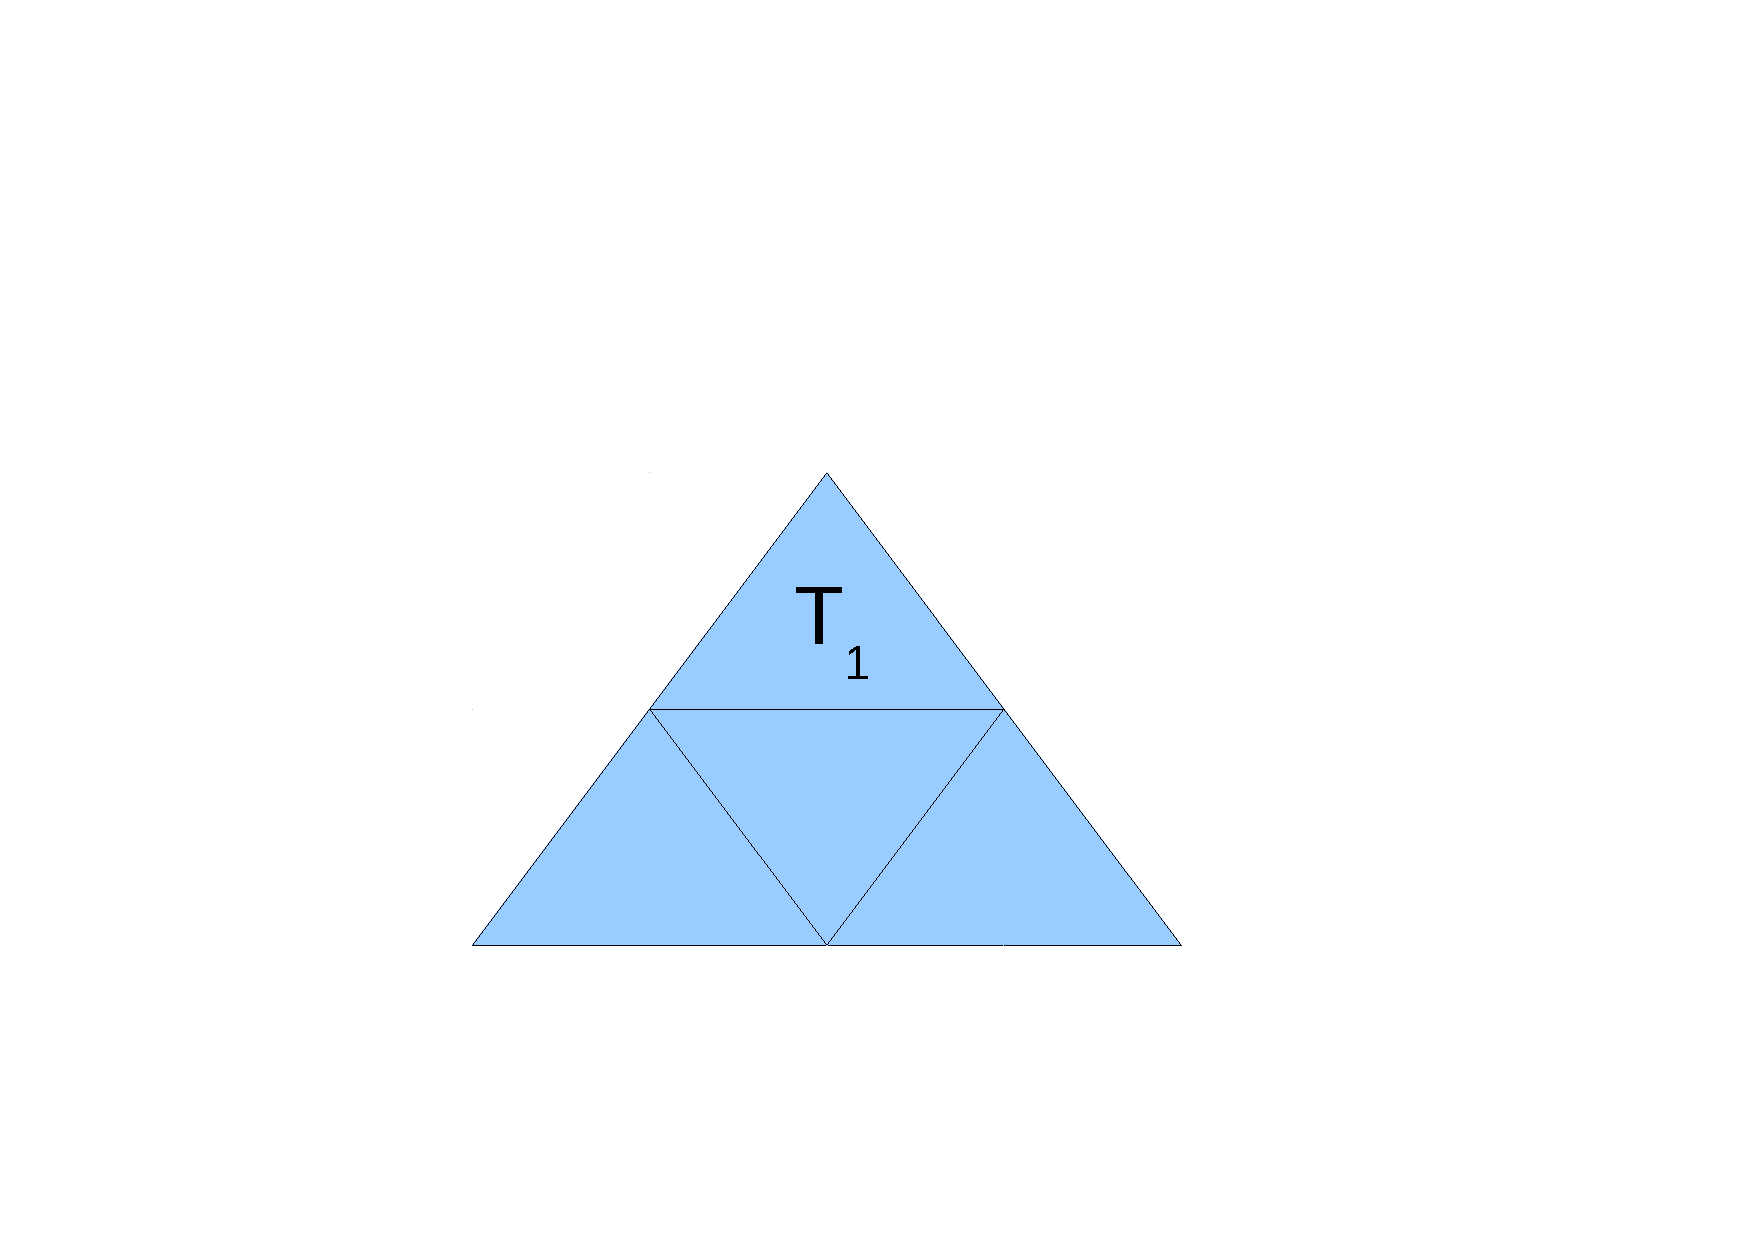
\includegraphics[scale=0.3]{images/subdivision_triangle.pdf}
\caption{Passage de $T_0$ à $T_1$ par subdivision}\label{fig:sub_triang}
\end{center}
\end{figure}

Si $L$ est le périmètre du triangle $T_0$, alors le périmètre du triangle $T_1$ est $L/2$, et par récurrence : à l'étape $n$ il y a $4^n$ triangles de périmètre $L/2^n$. Soit $d$ le diamètre du triangle $T_0$ (diamètre du cercle circonscrit) alors le diamètre de $T_n$ est $d/2^n$.
Alors,
\[J=\int_{\partial T_0} f(z) \diff z= \sum_{i=1}^{4^n} \int_{\partial T_{n,i}} f(z) \diff z,\] 
où $T_{n,i}$ désigne un des $4^n$ triangles de la subdivision obtenue à la $n$\ieme{} étape. Il existe donc un $i_n$ tel que 
\[\Bigl \lvert \int_{\partial T_{i_n}} f(z) \diff z \Bigr \rvert \geq \frac{\lvert J \rvert}{4^n}.\]

On construit ainsi une suite décroissante de triangles emboîtés 
\[T_0 \supset T_{i_1} \supset \cdots \supset T_{i_n} \supset \cdots.\]
C'est une suite décroissante de compacts non vides dans le compact $T_0$, donc l'intersection est non vide ; soit $a$ un point dans cette intersection. 

Notons que ce point appartient à $\Omega$ et donc $f$ est dérivable en $a$, par hypothèse d'holomorphie. D'où pour $\epsilon > 0$, il existe $r >0$ tel que :
\[
\forall z \in D(a;r), \quad \lvert f(z)-f(a)-f^\prime(a)(z-a)\rvert  < \epsilon \lvert z-a\rvert
.\]

En choisissant $N$ suffisamment grand pour que $d/2^n <r$ pour tout $n \geq N$, tous les triangles $T_{n,i}$ sont inclus dans $D(a;r)$ d'où en notant que l'application  $z \mapsto f(a)+f^\prime(a)(z-a)$ est une fonction polynomiale en $z$,
donc admet une primitive globale. Son intégrale est donc nulle sur le
bord de chaque triangle de $T_n$ et on peut écrire :
\begin{align*}
 \left \lvert
\int_{\partial T_n} f(z) \diff z
\right \rvert & \leq  \int_{\partial T_n}  \lvert f(z)-f(a)-f^\prime(a)(z-a)\rvert \lvert \diff z \rvert+ \left \lvert \int_{\partial T_n} f(a)+f^\prime(a)(z-a) \diff z \right\rvert   \\
& \leq \int_{\partial T_n}  \lvert f(z)-f(a)-f^\prime(a)(z-a)\rvert \lvert \diff z\rvert\\
& \leq  \epsilon d L/4^n.
\end{align*}

On en conclut que $\lvert J \rvert \leq \epsilon  d L$, et comme  
$\epsilon$ est arbitraire, l'intégrale est nulle.
\end{proof}

Le théorème de Goursat est encore vrai si l'on suppose seulement l'holomorphie
sur $\Omega$ privé d'une droite et la continuité sur $\Omega$: si la droite en
question coupe un chemin triangulaire on se ramènera par continuité et
subdivision au cas précédent. Dans un domaine simplement connexe, on a le très important théorème suivant:

\begin{fthm}
Soit $\Omega$ un domaine \textbf{simplement connexe}. Soit $f$ une application \textbf{holomorphe}
dans $\mathbb{C}$. Alors $f$ admet une primitive le long de tout chemin de
$\Omega$ et l'intégrale de $f$ sur tout lacet de $\Omega$ est nulle. On a de plus, une primitive globale $F$ de $f$ dans $\Omega$ donnée, pour tout $z_1 \in \Omega$, par~:
\[F(z_1)= F(z_0) + \int_\gamma f(z) \diff z,\]
où $z_0 \in \Omega$ et $\gamma$ est un chemin,  dans $\Omega$, d'origine $z_0$ et d'extrémité $z_1$. Le choix du point $z_0$ est arbitraire.


\end{fthm}

\begin{proof}
Le théorème de Goursat montre l'existence d'une primitive pour $f$ le long de
tout chemin de $\Omega$. Le domaine étant simplement connexe, tout lacet est
homotope à un lacet constant: l'intégrale de $f$ le long de tout lacet est
nulle.
\end{proof}

Le théorème qui vient d'être énoncé permet de calculer des intégrales de la
variable réelle difficiles à obtenir de façon directe. L'idée est de :
\begin{enumerate}
    \item prolonger $f(x)$ en une application analytique $f(z)$ dans un domaine englobant un intervalle $[-R,R]$ de l'axe réel,
    \item définir un lacet simple contenant cet intervalle et délimitant un domaine ne contenant aucune singularité de $f(z)$ (la composante connexe bornée du théorème de Jordan),
    \item calculer la valeur de l'intégrale sur la partie du lacet autre que l'intervalle, lorsque $R \to \infty$,
    \item enfin, en déduire la valeur de l'intégrale sur l'axe réel en faisant tendre $R \to \infty$.
\end{enumerate}
Notons que l'intégrale ainsi obtenue est une intégrale généralisée de Riemann. 

L'exercice suivant illustre la démarche pour l'évaluation des intégrales de Fresnel, que l'on rencontre assez fréquemment en physique.
\begin{exercice}
Soit l'application $f(z)=\exp\left(i z^2\right)$. 
\begin{itemize}
  \item Montrer que $f$ est holomorphe sur $\mathbb{C}$.
  \item Pour tout réel $r > 0$, le contour $\gamma_r$ est défini selon la figure
  \ref{fig:contour2}. Donner la valeur de l'intégrale:
  \[
  \int_{\gamma_r} f(z) \diff z.
  \]
  \item Écrire cette intégrale sous la forme d'une somme de trois
  intégrales de chemin et montrer que l'intégrale correspondant à l'arc de
  cercle tend vers $0$ lorsque $r \to +\infty$ (utiliser le lemme de Jordan par ex.).
  \item En déduire les valeurs des intégrales généralisées suivantes, dites
  intégrales de Fresnel:
  \[
  \lim_{r \to +\infty} \int_{[-r,r]} \cos(x^2) \diff x, \qquad  \lim_{r \to +\infty}
  \int_{[-r,r]} \sin(x^2) \diff x
  \]
\end{itemize}

\begin{figure}[H]
\begin{center}
\shorthandoff{!}\shorthandoff{:}
\begin{tikzpicture}[line cap=round,line join=round,>=triangle 45,x=1.0cm,y=1.0cm]

 \tikzset{
  % style to apply some styles to each segment of a path
  on each segment/.style={
    decorate,
    decoration={
      show path construction,
      moveto code={},
      lineto code={
        \path [#1]
        (\tikzinputsegmentfirst) -- (\tikzinputsegmentlast);
      },
      curveto code={
        \path [#1] (\tikzinputsegmentfirst)
        .. controls
        (\tikzinputsegmentsupporta) and (\tikzinputsegmentsupportb)
        ..
        (\tikzinputsegmentlast);
      },
      closepath code={
        \path [#1]
        (\tikzinputsegmentfirst) -- (\tikzinputsegmentlast);
      },
    },
  },
  % style to add an arrow in the middle of a path
  mid arrow/.style={postaction={decorate,decoration={
        markings,
        mark=at position .5 with {\arrow[#1]{stealth}}
      }}},
}   
 
\clip(-1,-1) rectangle (4,4);

\draw[->] (0,0) -- (3,0);
\draw (3,0) node[right] {$x$};
\draw [->] (0,0) -- (0,3);
\draw (0,3) node[above] {$y$}; 
\draw [line width=1.2pt,color=pblue, postaction={on each segment={mid arrow=red}}] (0,0) -- (2,0)  ;
\draw[line width=1.2pt,color=pblue, postaction={on each segment={mid arrow=red}}] (2,0) arc(0:45:2) -- (0,0) ;
\draw [fill=black] (0,0) circle (2pt);
\draw (0,0) node[left]{$0$} ;
 \draw [fill=black] (2,0) circle (2pt);
 \draw (2,0) node[below]{$r$} ;
\end{tikzpicture}
\shorthandon{!}\shorthandoff{:}
\caption{Chemin d'intégration pour le calcul des intégrales de Fresnel.}\label{fig:contour2}
\end{center}
\end{figure}



\end{exercice}
% \begin{figure}[ht]
%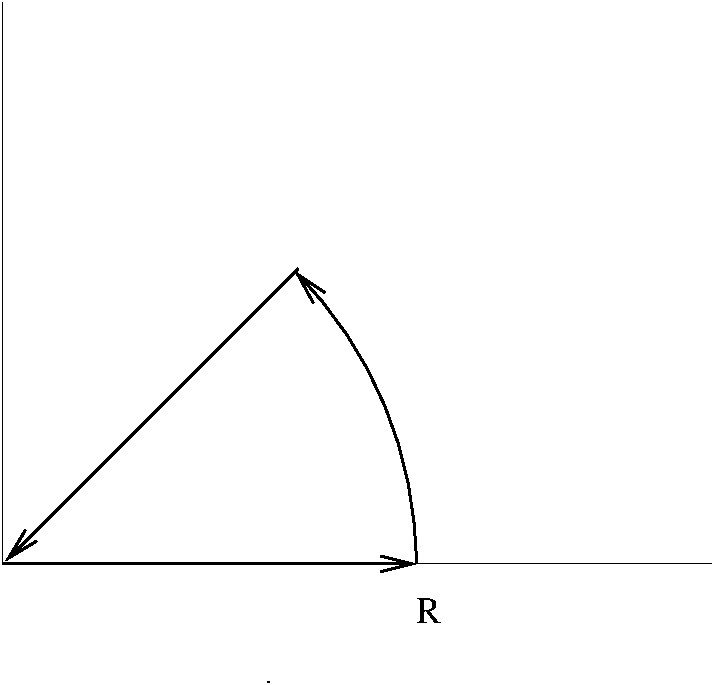
\includegraphics[scale=0.3]{images/contour_fresnel.pdf}
%\caption{Contour $\gamma_r$}\label{fig:contour2}
%\end{figure}
On utilise fréquemment les techniques d'intégration dans le plan complexe pour
obtenir des transformées de Fourier, c'est à dire calculer pour une fonction $f$ intégrable sur $\R$ au sens de Lebesgue ($f \in L^1(\R)$) l'application 
\[\hat{f}(\omega)= \int_{-\infty}^\infty f(t) e^{- i \omega t} \diff t. \]
L'exercice suivant calcule la transformée de Fourier de $f(x) = e^{-x^2}$. 
\begin{exercice}\label{exerGauss} 
Soit $f(z)=\exp(-z^2)$.
\begin{itemize}
  \item Montrer que $f$ est holomorphe dans $\mathbb{C}$.
  \item En utilisant le contour $\gamma$ donné en figure~\ref{fig:contour3}, déterminer la valeur de l'intégrale:
  \[\int_{\gamma} \exp(-z^2)dz.\]
  \item En faisant tendre $r$ vers $+\infty$ et en faisant un raisonnement
  similaire à celui de l'exercice précédent, déterminer la transformée de
  Fourier de l'application $x \mapsto \exp(-x^2)$.
\end{itemize}

\begin{figure}[H]
\begin{center}
\shorthandoff{!}\shorthandoff{:}
\begin{tikzpicture}[line cap=round,line join=round,>=triangle 45,x=1.0cm,y=1.0cm]

 \tikzset{
  % style to apply some styles to each segment of a path
  on each segment/.style={
    decorate,
    decoration={
      show path construction,
      moveto code={},
      lineto code={
        \path [#1]
        (\tikzinputsegmentfirst) -- (\tikzinputsegmentlast);
      },
      curveto code={
        \path [#1] (\tikzinputsegmentfirst)
        .. controls
        (\tikzinputsegmentsupporta) and (\tikzinputsegmentsupportb)
        ..
        (\tikzinputsegmentlast);
      },
      closepath code={
        \path [#1]
        (\tikzinputsegmentfirst) -- (\tikzinputsegmentlast);
      },
    },
  },
  % style to add an arrow in the middle of a path
  mid arrow/.style={postaction={decorate,decoration={
        markings,
        mark=at position .5 with {\arrow[#1]{stealth}}
      }}},
}   

\clip(-3,-1) rectangle (3,2.5);

\draw[->] (-3,0) -- (3,0);
\draw (3,0) node[right] {$x$};
\draw [->] (0,-0.5) -- (0,2);
\draw (0,3) node[above] {$y$}; 
\draw [line width=1.2pt,color=pblue, postaction={on each segment={mid arrow=red}}] (-2,0) -- (2,0)  ;
\draw[line width=1.2pt,color=pblue, postaction={on each segment={mid arrow=red}}] (2,0)  -- (2,0.8) ;
\draw[line width=1.2pt,color=pblue, postaction={on each segment={mid arrow=red}}] (2,0.8)  -- (-2,0.8) ;
\draw[line width=1.2pt,color=pblue, postaction={on each segment={mid arrow=red}}] (-2,0.8)  -- (-2,0) ;
%\draw [fill=black] (0,0) circle (2pt);
\draw (0,0) node[below left ]{$0$} ;
 \draw [fill=black] (2,0) circle (2pt);
 \draw (2,0) node[below]{$r$} ;
 \draw [fill=black] (-2,0) circle (2pt);
 \draw (-2,0) node[below]{$-r$} ;
 %\draw [fill=black] (0,0.8) circle (2pt);
 \draw (0,0.8) node[above right]{$i \frac{\omega}{2}$} ; 
\end{tikzpicture} 
\shorthandon{!}\shorthandoff{:} 
\caption{Contour $\gamma$ pour le calcul de la TF de $x \mapsto e^{-x^2}$.}\label{fig:contour3} 
\end{center} 
\end{figure} 

\end{exercice} 
 
%Nous avons vu qu'une forme différentielle $f(z) \diff z$ est fermée lorsque $f$ est holomorphe. Pour qu'elle soit exacte, il suffit donc que le domaine, sur laquelle est considérée cette forme, soit simplement connexe.  
 
\section{Formules de Cauchy}

\begin{fdefn}
Soit $\gamma$ un lacet et soit $z_0 \in \mathbb{C}$ n'appartenant pas à l'image
de $\gamma$. L'\textbf{indice} de $\gamma$ par rapport à $z_0$ est :
\[
I(\gamma;z_0) = \frac{1}{i 2 \pi}\int_{\gamma} \frac{1}{z-z_0} \diff z
\]
\end{fdefn}
L'indice d'un lacet compte le nombre de tours effectués par $\gamma$ autour de $z_0$, positivement dans le sens trigonométrique et négativement en sens opposé. Nous avons déjà calculé cette intégrale pour $z_0=0$ et $\gamma$, le cercle unité et obtenu la valeur $1$. Il faut montrer que l'indice est un entier. 

\begin{proof}
La preuve est celle de \cite{rudin1988analyse}. Nous avons
\[I(\gamma;z_0) = \frac{1}{i 2 \pi}\int_{[0,1]} \frac{\gamma^\prime(t)}{\gamma(t)-z_0} \diff t.\]
Or un complexe de la forme $\omega/(2 i \pi)$ est un entier si et seulement si $e^\omega=1$ ; il suffit donc de prouver que $\varphi(1)=1$ où 
\[\varphi(t)=\exp \left \{\int_0^t \frac{\gamma^\prime(u)}{\gamma(u)-z_0} \diff u \right\}.\]
On a $\frac{\varphi^\prime(t)}{\varphi(t)} = \frac{\gamma^\prime(t)}{\gamma(t)-z_0}$ sauf aux points où $\gamma$ n'est pas dérivable, qui sont en nombres finis. Ainsi, la fonction $\varphi(t)/(\gamma(t)-z_0)$ est continue et de dérivée nulle en dehors d'un nombre fini de points, donc $\varphi$ est constante. Par ailleurs, $\varphi(0) =1$, donc pour tout $t$, $ \varphi(t) = (\gamma(t) -z_0)/ (\gamma(0) -z_0)$. Comme $\gamma(1)=\gamma(0)$, nous obtenons que $\varphi(1)=1$.
\end{proof}




% On peut établir cette propriété en raisonnant en deux temps. Sans perte de généralité, on supposera que $z_0 = 0$. On note tout d'abord que si $\gamma$ ne passe pas par 0, il existe une boule fermée $B(0,r)$ ne rencontrant pas $\gamma$. L'application:
%\[
%H \colon (s,t) \in [0,1] \times [0,1] \mapsto s \frac{r \gamma(t)}{|\gamma(t)|} + (1-s) \gamma(t)
%\] 
%établit une homotopie dans $C^*$ entre $\gamma$ et un lacet $\tilde{\gamma} = H(1,\bullet)$ dont l'image appartient au cercle $\mathcal{C}_r$ de centre 0 et de rayon $r$. En vertu du théorème d'invariance homotopique, l'indice de $\tilde{\gamma}$ est le même que celui de $\gamma$. Au voisinage de $\mathcal{C}_r$, l'application:
%\[
%\ln \left(z = |z|\exp(i \theta) \right) = \ln |z| + i (\theta+ 2 k \pi), \theta \in [0, 2 \pi [ , k \in \Z
%\]
%définit une primitive locale de l'application $z^{-1}$ et la conclusion s'ensuit (faire un dessin et propager les écarts angulaires \dots). 


L'invariance par homotopie de l'intégrale montre que si $\gamma_1$ et $\gamma_2$ sont deux lacets homotopes dans $\C \setminus \{z_0\}$, alors $I(\gamma_1 ; z_0) = I(\gamma_2 ; z_0)$.

On peut également fixer $\gamma$ et faire varier le point $z_0$. La représentation de l'indice comme une intégrale, montre que l'indice dépend analytiquement du point $z_0 \in \C \setminus \gamma$ ; l'indice étant un entier, il est donc constante sur chaque composante connexe de $\C \setminus \gamma$. Comme l'intégrale tend vers $0$  lorsque $z_0 \to  \infty$, l'entier $I(\gamma ; z_0)$ est nul sur la composante connexe non bornée (cf. figure~\ref{fig:windingnumber}).

\begin{figure}[H]
\begin{center}
\shorthandoff{!}\shorthandoff{:}
\begin{tikzpicture}
%\tikzset{
%    on each segment/.style={
%        decorate,
%        decoration={
%            show path construction,
%            moveto code={},
%            lineto code={
%                \path [#1]
%                (\tikzinputsegmentfirst) -- (\tikzinputsegmentlast);
%            },
%            curveto code={
%                \path [#1] (\tikzinputsegmentfirst)
%                .. controls
%                (\tikzinputsegmentsupporta) and (\tikzinputsegmentsupportb)
%                ..
%                (\tikzinputsegmentlast);
%            },
%            closepath code={
%                \path [#1]
%                (\tikzinputsegmentfirst) -- (\tikzinputsegmentlast);
%            },
%        },
%    },
%     % style to add an arrow in the middle of a path
%  mid arrow/.style={postaction={decorate,decoration={
%        markings,
%        mark=at position .5 with {\arrow[#1]{stealth}}
%      }}},
%}
[decoration={markings,mark=at position 0.5 with {\arrow{>}}},
   witharrow/.style={postaction={decorate}},
   dot/.style={draw,fill,circle,inner sep=1.5pt,minimum width=0pt}
  ] 
 \begin{scope}[scale=2]   
\draw[witharrow,closed hobby, blue] plot coordinates {(0,0) (1,1) (0,1) (.5,.3) (.5,.7) (0,0)};    
 
  \draw [fill=black] (-1,0.5) circle (1pt);
 \draw (-1,0.5) node[below]{$z_0$} ;
 
 \draw [fill=black] (0.3,0.5) circle (1pt);
 \draw (0.3,0.5) node[below]{$z_2$} ;
 
 \draw [fill=black] (0.7,0.5) circle (1pt);
 \draw (0.7,0.5) node[below]{$z_1$} ;
 
 \end{scope}
    
    
\end{tikzpicture}

\shorthandon{!}\shorthandoff{:}

\caption{Les indices du chemin par à $z_0, z_1, z_2$ sont respectivement, $0,1$ et $2$.}\label{fig:windingnumber}
\end{center}
\end{figure}

\begin{fthm}(Première formule de Cauchy)\label{the:formcauchy}
Soit $\Omega$ un domaine simplement connexe de $\mathbb{C}$ et $f$ holomorphe
dans $\Omega$. Soit $\gamma$ un lacet de $\Omega$ et $z_0$ n'appartenant pas à
l'image de $\gamma$. On a:
\[
I(\gamma; z_0)f(z_0) = \frac{1}{2 \pi i}\int_{\gamma} \frac{f(z)}{z-z_0} \diff z.
\]
\end{fthm}
\begin{proof}
Soit l'application:
\[
F \colon z \mapsto \left \{
\begin{array}{cc} 
\frac{f(z)-f(z_0)}{z-z_0} & z \neq z_0 \\
f^\prime(z_0) & z = z_0
\end{array}
\right.
\]
$F$ est holomorphe dans $\Omega \setminus \{z_0\}$ et continue sur $\Omega$: le théorème
de Goursat (forme étendue) montre que l'intégrale de $F$ le long de $\gamma$ est
nulle, la conclusion est obtenue avec la proposition établie sur le calcul de
l'indice par intégrale curviligne.
\end{proof}

% La formule de Cauchy peut également s'énoncer dans le cas d'un domaine dont le
% bord est un lacet simple régulier de classe $C^1$ par morceaux:

% \begin{fprop}
% Soit $\Omega$ un domaine simplement connexe de bord $\partial \Omega$ un lacet simple de classe $C^1$ par morceaux et soit $f$ une application holomorphe dans $\Omega$ et continue sur $\Omega \cup \partial \Omega$. Pour tout point $z_0 \in \Omega$ on a :
% \[
% \frac{1}{2 \pi i} \int_{\partial \Omega} \frac{f(z)}{z-z_0} \diff z = f(z_0)
% \]
% \end{fprop}
 
% La preuve est similaire au cas précédent, mais utilise le théorème basé sur la
% formule de Stokes.
%  La formule de Cauchy se généralise immédiatement au cas d'un domaine
%  $n$-connexe dont le bord est constitué d'une union finie de lacets simples rectifiables, en se ramenant à un ouvert simplement connexe. On prendra
% garde néanmoins au sens de parcours du lacet.

\begin{rem} Exprimons l'intégrale de Cauchy pour $\gamma(t)=z_0 + r e^{i 2 \pi t}$ : le cercle de rayon $r$ centré en $z_0$, avec $r$ suffisamment petit de sorte que le support de $\gamma$ soit dans contenu dans $\Omega$. Nous obtenons  
\[f(z_0) = \frac{1}{2 \pi} \int\limits_{-\pi}^\pi f(z_0 + r e^{i \theta}) \diff \theta.\]
Ainsi $f(z_0)$ est la moyenne des valeurs de $f$ prises sur un cercle centré en $z_0$ ; cette propriété de la moyenne est une propriété caractéristique des fonctions harmoniques. Cette propriété, connue sous le nom de propriété de la valeur moyenne, s'étend aux fonctions harmoniques dans $\R^n$, pour $n$ quelconque. Elle implique en particulier le principe du maximum, qui stipule que le maximum (resp. le minimum) d'une fonction harmonique dans un domaine ne peut être atteint qu'en un point de la frontière de domaine \cite{axler2013harmonic}. 
\end{rem}

 \begin{fthm}(Seconde formule
de Cauchy) Sous les même hypothèses que celles du théorème~\ref{the:formcauchy}, on a~:
\[
I(\gamma; z_0) f^\prime(z_0) = \frac{1}{2 \pi i} \int_{\gamma}
\frac{f(z)}{(z-z_0)^2}\diff z.
\]
\end{fthm}

\begin{proof}
On supposera l'indice du lacet $\gamma$ égal à 1 pour simplifier les écritures.
Formons le rapport~:
\[
\frac{f(z_0+h)-f(z_0)}{h} = \frac{1}{2
\pi i}\int_{\gamma}\frac{f(z)}{(z-z_0)(z-z_0-h)} \diff z
\]
avec $h$ tel que $z_0+h \in \Omega$. En passant à la limite $|h|\to 0$, on
obtient le résultat par convergence dominée.
\end{proof}

Par récurrence, on obtient les dérivées d'ordre supérieur~:
\[
I(\gamma; z_0) f^{(n)}(z_0) = \frac{n!}{2 \pi i} \int_{\gamma}
\frac{f(z)}{(z-z_0)^{n+1}} \diff z.
\]
% Enfin, il est possible d'obtenir une formulation utilisant la formule de Stokes
% (la démonstration n'est pas détaillée).

% \begin{fthm}
% Soit $f$ holomorphe dans un domaine simplement connexe $\Omega$ dont le bord est un lacet simple de classe $C^1$ par morceaux. Si $f$ est continue sur
% $\partial \Omega$, elle est indéfiniment dérivable en tout $z_0 \in \Omega$ et~:
% \[
% f^{(n)}(z_0) =  \frac{n!}{2 \pi i} \int_{\partial \Omega} \frac{f(z)}{(z-z_0)^{n+1}} \diff z.
% \]
% \end{fthm}

Les formules intégrales de Cauchy montrent qu'une application holomorphe dans un
domaine y est indéfiniment dérivable. 

\begin{fcor}
Si $f(z)$ est holomorphe dans un domaine $\Omega$, alors $f$ est indéfiniment dérivable, et ses dérivées complexes successives, $f^\prime, f^{(2)}, \cdots$ sont aussi holomorphes dans $\Omega$.
\end{fcor}



\begin{exercice}
Soit $a>0$ réel et 
\[f(z) = \frac{e^{iaz}}{1+z^2}.\] 
\begin{itemize}
  \item En utilisant la première formule de Cauchy, évaluer l'intégrale de $f$
  le long du contour donné figure \ref{fig:contour_ex1}, sous l'hypothèse
  $R>1$ (pourquoi cette hypothèse ?).
  \item Par passage à la limite $R \to +\infty$, en déduire la transformée de
  Fourier de l'application $x \mapsto (1+x^2)^{-1}$.
\end{itemize}

\begin{figure}[H]
\begin{center}
\shorthandoff{!}\shorthandoff{:}
\begin{tikzpicture}[domain=0:4]

\tikzset{
  % style to apply some styles to each segment of a path
  on each segment/.style={
    decorate,
    decoration={
      show path construction,
      moveto code={},
      lineto code={
        \path [#1]
        (\tikzinputsegmentfirst) -- (\tikzinputsegmentlast);
      },
      curveto code={
        \path [#1] (\tikzinputsegmentfirst)
        .. controls
        (\tikzinputsegmentsupporta) and (\tikzinputsegmentsupportb)
        ..
        (\tikzinputsegmentlast);
      },
      closepath code={
        \path [#1]
        (\tikzinputsegmentfirst) -- (\tikzinputsegmentlast);
      },
    },
  },
  % style to add an arrow in the middle of a path
  mid arrow/.style={postaction={decorate,decoration={
        markings,
        mark=at position .5 with {\arrow[#1]{stealth}}
      }}},
}

\draw [<->, very thick] (0,4) node (yaxis) [above] {$y$}
    |- (-4,0) node (zaxis) [left] {}
    |- (4,0) node (xaxis) [right] {$x$}
    ;
   \path [color=blue,draw=black, ultra thick, postaction={on each segment={mid arrow=black}}] (3,0) arc (0:180:3cm)
    (-3,0) -> (3,0) ;
    \draw (-3,0) node[below]{$-R$};
    \draw (3,0) node[below]{\normalsize $R$};
%    (-1,0) arc (180:0:1cm) % changed starting point and swapped arc bounding angles
%    (-3,0) -> (-1,0) ; % swapped coordinates here



\end{tikzpicture}

\shorthandon{!}\shorthandoff{:}

\caption{Contour d'intégration}\label{fig:contour_ex1}
\end{center}
\end{figure}




\end{exercice}
%\begin{figure}[ht]
%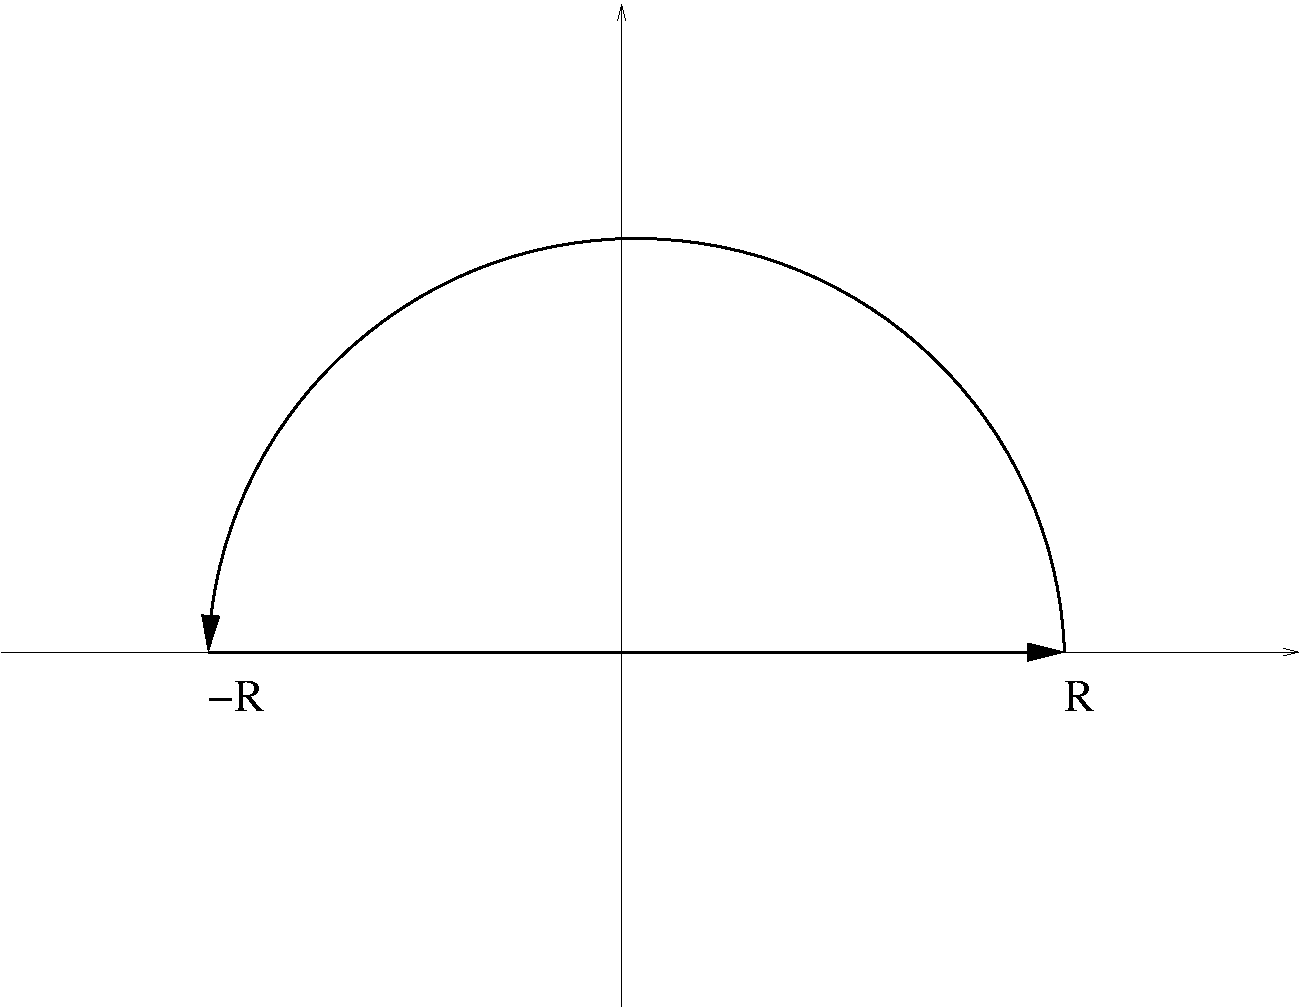
\includegraphics[scale=0.3]{images/contour_ex1.pdf}
%\caption{Contour d'intégration}\label{fig:contour_ex1}
%\end{figure}
\begin{exercice}
    En utilisant la première formule de Cauchy, calculer la valeur de l'intégrale:
    \[
    \int_0^{2\pi} \frac{1}{2 + \sin x} dx
    \]
    \leftline{\textbf{Indication:}}
    Écrire le sinus sous la forme:
    \[
\sin x =\frac{e^{ix}-e^{-ix}}{2i}
    \]
    et vérifier que l'intégrale précédente est une intégrale sur un lacet dans le plan
    complexe.
\end{exercice}

Supposons la fonction $f$ holomorphe dans un domaine contenant le disque fermé $\{\lvert z-z_0 \rvert \leq \rho \}$. Par la formule intégrale de Cauchy pour $f^{(n)}$,
\[ f^{(n)}(z_0) =  \frac{n!}{i 2 \pi} \int\limits_{\lvert z-z_0 \rvert = \rho } \frac{f(z)}{(z-z_0)^{n+1}} \diff z.
\]
Par paramétrisation du cercle frontière : $z=z_0 + \rho e^{i \theta}$, $\diff z = i \rho e^{i \theta} \diff \theta$, nous obtenons
\[f^{(n)}(z_0) =  \frac{n!}{\rho^n} \int_0^{2 \pi} f(z_0 + \rho e^{i \theta}) e^{-i n  \theta} \frac{\diff \theta}{2 \pi},\]
d'où la majoration suivante~:
\[\lvert f^{(n)}(z_0)\rvert \leq  \frac{n!}{\rho^n} \int_0^{2 \pi} \lvert f(z_0 + \rho e^{i \theta})\rvert  \frac{\diff \theta}{2 \pi}.\]
Ceci conduit aux inégalités de Cauchy suivantes :
\begin{prop}
Supposons que la fonction $f$ soit holomorphe dans un domaine contenant le disque fermé $\{\lvert z-z_0 \rvert \leq \rho \}$. Si $\lvert f(z) \rvert \leq M$ pour $\lvert z-z_0 \rvert =\rho $, alors
\[\lvert f^{(n)}(z_0)\rvert \leq \frac{n!}{\rho^n} M, \quad n \geq 0.\]
\end{prop}

Une application importante de ces inégalités est le théorème de Liouville
\begin{theorem}[Liouville]
Soit $f$ une fonction holomorphe dans $\C$ (donc une fonction entière). Si $f$ est bornée, alors $f$ est constante.
\end{theorem}
\begin{proof}
Supposons $f$ bornée par $M$ pour tout $z \in \C$. En appliquant l'inégalité de Cauchy sur un disque centré en $z_0$ quelconque et pour tout rayon $\rho$, on obtient que $\lvert f^\prime(z_0)\rvert \leq \frac{M}{\rho}$.
Lorsque $\rho$ tend vers $+\infty$, nous obtenons que $f^\prime(z_0)=0$, identité valable pour tout $z_0$, donc $f$ est constante.
\end{proof}
%\subsection{Calcul numérique}
%Le théorème de Stokes complexe peut être utilisé pour calculer 
%numériquement la surface du domaine $\Omega$ entouré par un lacet polygonal $\gamma$. Si 
%l'on se donne ce dernier par une liste de sommets $(z_i), \, i=0 \dots N-1$ on peut paramétrer le chemin liant le sommet $i$ au sommet $i+1$ comme:
%\[
%\gamma_i \colon t \in [0,1] \mapsto z_i + t\left(z_{i+1}-z_i\right)
%\]
%Sur cette partie du lacet, on formera l'intégrale:
%\[
%\int_{\gamma_i}\overline{z}dz = \int_{[0,1]}\left(\overline{ z_i}+t \overline{\left(z_{i+1}-z_i\right)}\right)\left(z_{i+1}-z_i\right) dt=
%\frac{\overline{z_{i+1}}+\overline{z_i}}{2}\left(z_{i+1}-z_i\right)
%\]
%et par la formule de Stokes complexe:
%\[
%\sum_{i=0}^{N-1}\frac{\overline{z_{i+1}}+\overline{z_i}}{2}\left(z_{i+1}-z_i\right) = - \int_{\Omega} dz d\overline{z}
%\]
%Comme:
%\[
%\int_{\Omega} dz d\overline{z} = - 2 i \int_{\Omega} dx dy
%\]
%on en déduit que la surface de $\Omega$ est égale à:
%\[
%- i \sum_{i=0}^{N-1}\frac{\overline{z_{i+1}}+\overline{z_i}}{4}\left(z_{i+1}-z_i\right)
%\]
%En développant, on obtient:
%\[
%- \frac{i}{4} \sum_{i=0}^{N-1} \left(\left|z_{i+1}\right|^2 - \left|z_i \right|^2 + 2 i \Im \left(z_{i+1}\overline{z_i} \right)
%\right)
%\]
%On peut vérifier sans difficultés que les termes en module carré se simplifient deux à deux dans la somme (se rappeler que $z_N = z_0$). La surface est donc en final:
%\[
%\frac{1}{2} \sum_{i=0}^{N-1} \Im \left(z_{i+1}\overline{z_i} \right)
%\]
%Enfin, on remarque que pour tout couple $(z_1=x_1+iy_1, z_2=x_2+iy_2)$ le produit $z_2 \overline{z_1}$ a pour partie réelle le produit scalaire des vecteurs $(x_1,y_1)$ et $(x_2,y_2)$ et pour partie réelle leur déterminant. Ceci donne une interprétation géométrique à la formule de sommation précédente, le déterminant de deux vecteurs orientés en sens direct s'identifiant à la surface du parallélogramme qu'ils définissent. Le code python ci-dessous implémente le calcul de surface tel qu'il vient d'être énoncé. 
%\begin{verbatim}
%# -*- coding: utf8 -*-
%import math
%
%
%# classe point
%class Point:
%    def __init__(self,x=0.0,y=0.0):
%        self.x=x
%        self.y=y
%# classe lacet
%class Lacet:
%    # constructeur. La liste de points est initialement vide
%    def __init__(self):
%        self.point_list=[]
%    # ajoute un point à la liste définissant le lacet
%    # p : point
%    def add(self,p):
%        self.point_list.append(p)
%    # calcule la surface entourée par le lacet
%    # return: réel
%    def surface(self):
%        surf = 0.0
%        n = len(self.point_list)-1
%        for i in range(n):
%            surf = surf-self.point_list[i+1].x*self.point_list[i].y\
%             + self.point_list[i+1].y * self.point_list[i].x
%        	surf = surf - self.point_list[0].x*self.point_list[n].y\
%        	 + self.point_list[0].y*self.point_list[n].x
%        return 0.5 * surf
%# test
%gamma=Lacet()
%gamma.add(Point(1.0,0.0))
%gamma.add(Point(0.0,1.0))
%gamma.add(Point(-1.0,0.0))
%gamma.add(Point(0.0,-1.0))
%
%print(gamma.surface())
%
%gamma=Lacet()
%gamma.add(Point(1.0,1.0))
%gamma.add(Point(-1.0,1.0))
%gamma.add(Point(-1.0,-1.0))
%gamma.add(Point(1.0,-1.0))
%
%print(gamma.surface())
%\end{verbatim}
%A titre d'exercice, améliorer le code pour inclure des lacets définis par des segments de droites et des arcs de cercle. 

\section{Exercices complémentaires}

\begin{exer}
L'objectif de cet exercice, extrait de \cite{lax2011complex}, est de prouver le théorème fondamental de l'algèbre qui affirme que tout polynôme non constant
\[p(z)=a_n z^n + a_{n-1}z^{n-1} + \cdots + a_0\]
avec des coefficients complexes doit s'annuler quelque part dans le plan complexe. On supposera dans la suite que $n \geq 1$ et $a_n \neq 0$.
\begin{MYenumerate}
\item Montrer que pour $\lvert z \rvert$ suffisamment grand, 
\[\lvert p(z)  \rvert  \geq  \lvert z^n  \rvert \left(\lvert a_n  \rvert -\lvert a_{n-1}\rvert/\lvert z\rvert  - \cdots -  \lvert a^{0}\rvert/\lvert z\rvert^n \right)> \frac{\lvert a_n\rvert}{2} \lvert z^n  \rvert.\]
En déduire que $\lim_{R \to \infty} \lvert p(R e^{i \theta}) \rvert = \infty$ uniformément en $\theta$.
\item Supposons que $p$ ne s'annule pas dans $\C$. Considérez la fonction $q=1/p$ et expliquer pourquoi elle est holomorphe dans $\C$ et que $q(0)  \neq 0$.
\item Appliquer la première formule de Cauchy à la fonction $q$ sur le cercle centré en $0$ et de rayon $R$, pour tout $R >0$. Puis faire tendre $R \to \infty$ pour aboutir à une contradiction.
\end{MYenumerate}
\end{exer}

\begin{exer}
\begin{MYenumerate}
\item Montrer que si $\gamma$ est un lacet simple entourant l'origine, alors 
\[\binom{n}{k} = \frac{1}{2 \pi i} \int_\gamma \frac{(1+z)^n}{z^{k+1}} \diff z.\]
\item En prenant pour lacet, le cercle unité, en déduire que 
\[\binom{2 n}{n} \leq 4^n.\]
\end{MYenumerate}
\end{exer}

\newpage 
\subsection*{Un peu d'histoire \dots}

\begin{minipage}{0.2\linewidth}
\begin{center}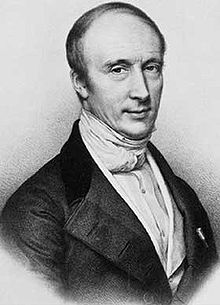
\includegraphics[width=2cm]{images/Cauchy.jpg}\end{center}
\end{minipage}
\begin{minipage}{0.80 \linewidth}
\small{\paragraph*{Augustin Louis Cauchy :} né le  né à Paris le 21 août 1789 et mort à Sceaux (Hauts-de-Seine) le 23 mai 1857. C'est un des mathématiciens les plus productifs connus (800 publications à son actif). Ses travaux ont concerné la plupart des domaines des mathématiques de son époque: analyse, algèbre, géométrie, probabilités. On lui doit le critère qui porte son nom pour les suites et est à l'origine de la théorie de l'intégration complexe.}
\end{minipage}

\vfill


\begin{minipage}{0.2\linewidth}
\begin{center}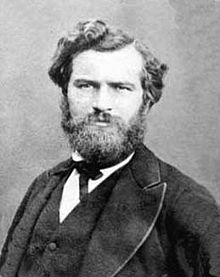
\includegraphics[width=2cm]{images/Jordan.jpg}\end{center}
\end{minipage}
\begin{minipage}{0.80\linewidth}
\small{\paragraph*{Camille Jordan :} né à Lyon le 5 Janvier 1838 et mort à Paris le 22 Janvier 1922. Ingénieur de formation, il enseigne les mathématiques à l'école polytechnique et au collège de France. On lui doit un remarquable cours d'analyse, ainsi que de nombreuses contributions en théorie des groupes.}
\end{minipage}
\vfill


\begin{minipage}{0.2\linewidth}
\begin{center}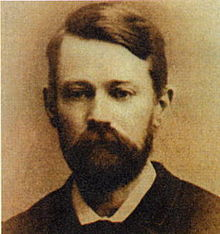
\includegraphics[width=2cm]{images/Stieltjes.jpg}\end{center}
\end{minipage}
\begin{minipage}{0.80\linewidth}
\small{\paragraph*{Thomas Joannes Stieltjes :} né le 29 décembre 1856 à Zwolle (Pays-Bas), mort le 31 décembre 1894 à Toulouse. Il travaillera sur les fractions continues, les formules de quadratures de Gauss et généralisera l'intégrale de Riemann.}
\end{minipage}

\vfill

\begin{minipage}{0.2\linewidth}
\begin{center}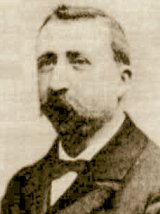
\includegraphics[width=2cm]{images/Goursat.jpg}\end{center}
\end{minipage}
\begin{minipage}{0.80 \linewidth}
\small{\paragraph*{Edouard Goursat :} né le 21 mai 1858 à Lanzac (Lot) et mort le 25 novembre 1936 à Paris. Il travailla sur les fonctions de la variable complexe et prouva le lemme qui porte son nom. Son cours d'analyse a été longtemps une référence.}
\end{minipage}

\vfill

\begin{minipage}{0.2\linewidth}
\begin{center}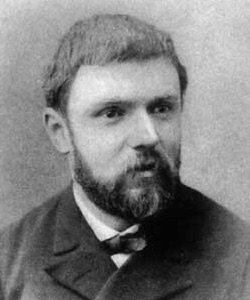
\includegraphics[width=2cm]{images/poincare.jpg}\end{center}
\end{minipage}
\begin{minipage}{0.80 \linewidth}
\small{\paragraph*{Henri Poincaré :} né le 29 avril 1854 à Nancy et mort le 17 juillet 1912 à Paris. Henri Poincaré fut le plus grand homme de sciences de la fin du XIX\ieme{} et du début du XX\ieme{} siècle, il est aussi le dernier à pouvoir comprendre l'ensemble des mathématiques de son époque et d'être en même temps un penseur philosophique (publication de la \og science et l'hypothèse\fg{} en 1902). Poincaré est le fondateur de la topologie algébrique. Ses principaux travaux mathématiques ont eu pour objet la géométrie algébrique, les fonctions dites\og automorphes \fg{} (il découvre les fonctions fuchsiennes et kleinéennes), les équations différentielles. Il étudie le problème des trois corps dans le cadre d'un concours organisé par Gosta Mittag-Leffler, Poincaré démontre qu'il n'y a pas de solutions générales et pose les prémisses de la théorie du chaos. Une conjecture posée en 1904 par Poincaré, et qui porte son nom, a été démontré par Grigori Perelman en 2003 ; elle concernait la sphère de dimension $3$. }
\end{minipage}